% Template de LaTex para tesis del ITESM Campus Guadalajara
% Basado en el template de Word de Ra'ul Crespo Saucedo
% Basado en el sistema de guiones de Universidad Computense de Madrid
% Adaptaci'on realizada por Arturo Jafet Rodr'iguez Mu'noz
% Revision por Marco Antonio Rangel Bocardo
% Maestr'ia en Ciencias Computacionales - ITESM Campus Guadalajara
% Guadalajara, Jalisco Septiembre del 2011
% Recomiendo esta gu'ia de LaTex: http://en.wikibooks.org/wiki/LaTeX/

\documentclass[12pt,letterpaper]{report}
\usepackage[english,spanish,activeacute]{babel}
\usepackage[T1]{fontenc}
\usepackage{dirtytalk}
\usepackage{graphicx}
\usepackage[letterpaper]{geometry}
\usepackage{titlesec}
\usepackage{fancyhdr}
\usepackage{fix-cm}
\usepackage{setspace} 
\usepackage{amsmath}
\usepackage{fmtcount}
\usepackage{threeparttable}
\usepackage{float}
\usepackage{mathtools}

\usepackage{graphicx}
\usepackage[table]{xcolor}
\usepackage{listings}

\usepackage[font=small,format=plain,labelfont=bf,it]{caption}
\geometry{top=2.5cm, bottom=2.5cm, left=3.0cm, right=2.5cm}
\renewcommand{\rmdefault}{cmr} % Roman
\renewcommand{\encodingdefault}{T1}
\newcommand{\subscript}[1]{\ensuremath{_{\textrm{#1}}}}
\setstretch{1.5}

\usepackage{hyperref}


%\headheight = 49pt
%\footskip = 10pt


%----------------------------------------------------------------
%
% Fichero con algunas divisiones de palabras que LaTeX no
% hace correctamente si no se le da alguna ayuda.
%
% Universidad Computense de Madrid
% http://gaia.fdi.ucm.es/projects/texis
%----------------------------------------------------------------

\hyphenation{
% a
abs-trac-to
abs-trac-tos
abs-trac-ta
abs-trac-tas
ac-tua-do-res
a-gra-de-ci-mien-tos
ana-li-za-dor
an-te-rio-res
an-te-rior-men-te
apa-rien-cia
a-pro-pia-do
a-pro-pia-dos
a-pro-pia-da
a-pro-pia-das
a-pro-ve-cha-mien-to
a-que-llo
a-que-llos
a-que-lla
a-que-llas
a-sig-na-tu-ra
a-sig-na-tu-ras
a-so-cia-da
a-so-cia-das
a-so-cia-do
a-so-cia-dos
au-to-ma-ti-za-do
% b
batch
bi-blio-gra-f\'ia
bi-blio-gr\'a-fi-cas
bien
bo-rra-dor
boo-l-ean-expr
% c
ca-be-ce-ra
call-me-thod-ins-truc-tion
cas-te-lla-no
cir-cuns-tan-cia
cir-cuns-tan-cias
co-he-ren-te
co-he-ren-tes
co-he-ren-cia
co-li-bri
co-men-ta-rio
co-mer-cia-les
co-no-ci-mien-to
cons-cien-te
con-si-de-ra-ba
con-si-de-ra-mos
con-si-de-rar-se
cons-tan-te
cons-trucci\'on
cons-tru-ye
cons-tru-ir-se
con-tro-le
co-rrec-ta-men-te
co-rres-pon-den
co-rres-pon-dien-te
co-rres-pon-dien-tes
co-ti-dia-na
co-ti-dia-no
crean
cris-ta-li-zan
cu-rri-cu-la
cu-rri-cu-lum
cu-rri-cu-lar
cu-rri-cu-la-res
% d
de-di-ca-do
de-di-ca-dos
de-di-ca-da
de-di-ca-das
de-rro-te-ro
de-rro-te-ros
de-sa-rro-llo
de-sa-rro-llos
de-sa-rro-lla-do
de-sa-rro-lla-dos
de-sa-rro-lla-da
de-sa-rro-lla-das
de-sa-rro-lla-dor
de-sa-rro-llar
des-cri-bi-re-mos
des-crip-ci\'on
des-crip-cio-nes
des-cri-to
des-pu\'es
de-ta-lla-do
de-ta-lla-dos
de-ta-lla-da
de-ta-lla-das
di-a-gra-ma
di-a-gra-mas
di-se-�os
dis-po-ner
dis-po-ni-bi-li-dad
do-cu-men-ta-da
do-cu-men-to
do-cu-men-tos
% e
edi-ta-do
e-du-ca-ti-vo
e-du-ca-ti-vos
e-du-ca-ti-va
e-du-ca-ti-vas
e-la-bo-ra-do
e-la-bo-ra-dos
e-la-bo-ra-da
e-la-bo-ra-das
es-co-llo
es-co-llos
es-tu-dia-do
es-tu-dia-dos
es-tu-dia-da
es-tu-dia-das
es-tu-dian-te
e-va-lua-cio-nes
e-va-lua-do-res
exis-ten-tes
exhaus-ti-va
ex-pe-rien-cia
ex-pe-rien-cias
% f
for-ma-li-za-do
% g
ge-ne-ra-ci\'on
ge-ne-ra-dor
ge-ne-ra-do-res
ge-ne-ran
% h
he-rra-mien-ta
he-rra-mien-tas
% i
i-dio-ma
i-dio-mas
im-pres-cin-di-ble
im-pres-cin-di-bles
in-de-xa-do
in-de-xa-dos
in-de-xa-da
in-de-xa-das
in-di-vi-dual
in-fe-ren-cia
in-fe-ren-cias
in-for-ma-ti-ca
in-gre-dien-te
in-gre-dien-tes
in-me-dia-ta-men-te
ins-ta-la-do
ins-tan-cias
% j
% k
% l
len-gua-je
li-be-ra-to-rio
li-be-ra-to-rios
li-be-ra-to-ria
li-be-ra-to-rias
li-mi-ta-do
li-te-ra-rio
li-te-ra-rios
li-te-ra-ria
li-te-ra-rias
lo-tes
% m
ma-ne-ra
ma-nual
mas-que-ra-de
ma-yor
me-mo-ria
mi-nis-te-rio
mi-nis-te-rios
mo-de-lo
mo-de-los
mo-de-la-do
mo-du-la-ri-dad
mo-vi-mien-to
% n
na-tu-ral
ni-vel
nues-tro
% o
obs-tan-te
o-rien-ta-do
o-rien-ta-dos
o-rien-ta-da
o-rien-ta-das
% p
pa-ra-le-lo
pa-ra-le-la
par-ti-cu-lar
par-ti-cu-lar-men-te
pe-da-g\'o-gi-ca
pe-da-g\'o-gi-cas
pe-da-g\'o-gi-co
pe-da-g\'o-gi-cos
pe-rio-di-ci-dad
per-so-na-je
plan-te-a-mien-to
plan-te-a-mien-tos
po-si-ci\'on
pre-fe-ren-cia
pre-fe-ren-cias
pres-cin-di-ble
pres-cin-di-bles
pri-me-ra
pro-ble-ma
pro-ble-mas
pr\'o-xi-mo
pu-bli-ca-cio-nes
pu-bli-ca-do
% q
% r
r\'a-pi-da
r\'a-pi-do
ra-zo-na-mien-to
ra-zo-na-mien-tos
re-a-li-zan-do
re-fe-ren-cia
re-fe-ren-cias
re-fe-ren-cia-da
re-fe-ren-cian
re-le-van-tes
re-pre-sen-ta-do
re-pre-sen-ta-dos
re-pre-sen-ta-da
re-pre-sen-ta-das
re-pre-sen-tar-lo
re-qui-si-to
re-qui-si-tos
res-pon-der
res-pon-sa-ble
% s
se-pa-ra-do
si-guien-do
si-guien-te
si-guien-tes
si-guie-ron
si-mi-lar
si-mi-la-res
si-tua-ci\'on
% t
tem-pe-ra-ments
te-ner
trans-fe-ren-cia
trans-fe-ren-cias
% u
u-sua-rio
Unreal-Ed
% v
va-lor
va-lo-res
va-rian-te
ver-da-de-ro
ver-da-de-ros
ver-da-de-ra
ver-da-de-ras
ver-da-de-ra-men-te
ve-ri-fi-ca
% w
% x
% y
% z
}
% Variable local para emacs, para que encuentre el fichero
% maestro de compilaci\'on
%%%
%%% Local Variables:
%%% mode: latex
%%% TeX-master: "./Tesis.tex"
%%% End:


\begin{document}
	\renewcommand{\tablename}{Tabla}

	\pagestyle{empty}
\begin{center}
\begin{center}

\includegraphics[scale=0.5]{images/escudo-itesm_small.png}
\end{center}
\vspace{17 pt}
\renewcommand{\baselinestretch}{1.0}
\Huge
%\textbf{I\hspace{1pt}n\hspace{1pt}s\hspace{1pt}t\hspace{1pt}i\hspace{1pt}t\hspace{1pt}u\hspace{1pt}t\hspace{1pt}o\hspace{1pt} \hspace{1pt}T\hspace{1pt}e\hspace{1pt}c\hspace{1pt}n\hspace{1pt}o\hspace{1pt}l\hspace{1pt}'o\hspace{1pt}g\hspace{1pt}i\hspace{1pt}c\hspace{1pt}o\hspace{1pt} \hspace{1pt}y \hspace{1pt}d\hspace{1pt}e\hspace{1pt} \hspace{1pt}E\hspace{1pt}s\hspace{1pt}t\hspace{1pt}u\hspace{1pt}d\hspace{1pt}i\hspace{1pt}o\hspace{1pt}s\\ S\hspace{1pt}u\hspace{1pt}p\hspace{1pt}e\hspace{1pt}r\hspace{1pt}i\hspace{1pt}o\hspace{1pt}r\hspace{1pt}e\hspace{1pt}s\hspace{1pt} \hspace{1pt}d\hspace{1pt}e\hspace{1pt} \hspace{1pt}M\hspace{1pt}o\hspace{1pt}n\hspace{1pt}t\hspace{1pt}e\hspace{1pt}r\hspace{1pt}r\hspace{1pt}e\hspace{1pt}y}\\
\textbf{Instituto Tecnol'ogico y de Estudios\\Superiores de Monterrey}\\
\LARGE
\textbf{Campus Guadalajara}\\
\vspace{11 pt}

\Large
\textbf{Escuela de Graduados en Ingenier'ia y\\ Arquitectura (EGIA)}\\
\vspace{20 pt}

\textbf{Maestr'ia en Ciencias Computacionales}\\
\vspace{42 pt}

\Huge
\textbf{Methodology for design of self sustainable IoT network}\\
\vspace{65 pt}

\Large
\begin{flushleft}
\hspace{5pt}\textbf{AUTOR: Victor Manuel Rodriguez Bahena}\\
\vspace{5pt}
\hspace{5pt}\textbf{ASESORES:PhD Marcos de Alba} \\
\end{flushleft}

\large
\vspace{20pt}
\textbf{Guadalajara (Jal), 10 de Mayo de 2015}
\end{center}
\clearpage

\renewcommand{\baselinestretch}{1.5}


	\pagenumbering{roman}
	%Empieza configuracion
\setstretch{1.0}
\titleformat{\chapter}{\Huge\bfseries}{\thechapter}{0 pt}{\rule{340 pt}{3 pt}\\}
\titlespacing{\chapter}{100 pt}{-25 pt}{40 pt}[10 pt]	
\pagestyle{fancy}
\fancyhead[RO,RE]{\thepage}
\fancyfoot[CO,CE]{}
%Termina configuracion

\chapter*{Acknowledgments}
\addcontentsline{toc}{chapter}{Acknowledgments}
\setstretch{1.5} %Regresa el interlineado a 1.5

\vspace{140 pt}

\normalsize
\begin{flushright}
\textit{First and foremost, I have to thank my parents for their love and support
throughout my life. My brother and loved ones deserve my wholehearted thanks as
well. Thank you for your understanding, patience and encouragement in many
difficult moments.}

\textit{I would like to express my sincere gratitude to my advisor PhD.
Marcos Ruben de Alba Rosano for the continuous support of my master degree 
study and related research, for  his patience, motivation,
and immense knowledge.}

\textit{I would like to sincerely thank Intel company as well as the Instituto
Tecn\'ologico y de Estudios Superiores de Monterrey for his support with the
scholarship and support to finish this achievement in my life.}

\end{flushright}
\clearpage

	%Empieza configuracion
\setstretch{1.0}
\titleformat{\chapter}{\Huge\bfseries}{\thechapter}{0 pt}{\rule{340 pt}{3 pt}\\}
\titlespacing{\chapter}{100 pt}{-25 pt}{40 pt}[10 pt]	
\pagestyle{fancy}
\fancyhead[RO,RE]{\thepage}
\fancyfoot[CO,CE]{}
%Termina configuracion

\chapter*{Acknowledgments}
\addcontentsline{toc}{chapter}{Acknowledgments}
\setstretch{1.5} %Regresa el interlineado a 1.5

\normalsize
\noindent
\clearpage

	%Empieza configuracion
\setstretch{1.0}
\titleformat{\chapter}{\Huge\bfseries}{\thechapter}{0 pt}{\rule{340 pt}{3 pt}\\}
\titlespacing{\chapter}{100 pt}{-25 pt}{40 pt}[10 pt]	
\pagestyle{fancy}
\fancyhead[RO,RE]{\thepage}
\fancyfoot[CO,CE]{}
%Termina configuracion

\chapter*{Resumen}
\addcontentsline{toc}{chapter}{Resumen}
\setstretch{1.5} %Regresa el interlineado a 1.5


\normalsize
\noindent El resumen es una s'intesis de la tesis. Generalmente incluir'a la definici'on del problema, el procedimiento o m'etodos, los resultados y las conclusiones. Esta secci'on deber'a tener un m'aximo de trescientas cincuenta palabras incluyendo preposiciones. Las palabras en el t'itulo no se cuentan como parte del resumen. El resumen debe escribirse con claridad, ya que 'esta es la referencia que se hace p'ublica inmediatamente en los servicios electr'onicos de b'usqueda de informaci'on. Deber'a escribirse a doble espacio. No se recomienda usar diagramas ni f'ormulas en esta secci'on.

En este documento se presenta la estructura de la propuesta de tesis que los alumnos del curso Seminario de Innovaci'on y Creatividad deben presentar para acreditar la materia. Se describen los elementos de la propuesta y el formato que dichos elementos deben llevar. En la portada debe ir el t'itulo tentativo de la tesis, el nombre del autor, la instituci'on de educaci'on superior en la que se realiza el trabajo de tesis, el mes y a'no en que se entreg'o la propuesta. Despu'es de la portada va una p'agina de aprobaci'on que debe ser firmada por el director de la tesis y los sinodales una vez el proyecto haya sido aprobado. En el caso que el documento sea una propuesta de tesis, se debe llenar el formato de Registro de Tesis que se debe entregar a Servicios Escolares antes de que termine el seminario. Este Registro es una condici'on necesaria para que el alumno pueda inscribirse a la materia que sigue: Tesis I.

Posteriormente, puede seguir una dedicatoria que es de car'acter opcional y una secci'on de reconocimientos en la que deben mencionarse aquellas instituciones o personas, si las hay, que est'en proporcionando ayuda o apoyo financiero al proyecto. Por 'ultimo sigue el resumen de la tesis, cuya extensi'on debe ser de una p'agina a dos p'aginas m'aximo.

El contenido muestra las diferentes secciones y cap'itulos de la tesis. Las p'aginas se indican con numeraci'on ar'abiga comenzando desde el cap'itulo 1. Las p'aginas de todas las secciones anteriores al cap'itulo 1 se identifican con numeraci'on romana. Si se usaron tablas o figuras en la tesis, deben incluirse las listas correspondientes de tablas o figuras despu'es de la secci'on de contenido.

Los cap'itulos de introducci'on, desarrollo y conclusiones vienen despu'es, numerados a partir del n'umero 1, con las referencias de cada cap'itulo puestas al final del mismo usando el formato del Institute of Electrical and Electronics Engineers (IEEE). Los ap'endices se identifican con letras (Ap'endice A, Ap'endice B, etc.), y tambi'en pueden llevar referencias bibliogr'aficas. Finalmente, puede haber una s'intesis biogr'afica del autor de tesis.
\clearpage

	\renewcommand{\baselinestretch}{1}
\titleformat{\chapter}{\Huge\bfseries}{\thechapter}{0 pt}{\rule{340 pt}{3 pt}\\}
\titlespacing{\chapter}{100 pt}{-25 pt}{40 pt}[10 pt]	
\renewcommand{\baselinestretch}{1.5}
\renewcommand{\contentsname}{Contenido} 
\tableofcontents
\renewcommand{\baselinestretch}{1.5}
	\renewcommand{\baselinestretch}{1}
\titleformat{\chapter}{\Huge\bfseries}{\thechapter}{0 pt}{\rule{340 pt}{3 pt}\\}
\titlespacing{\chapter}{100 pt}{-49 pt}{40 pt}[10 pt]	
\renewcommand{\listtablename}{Lista de Tablas} 
\listoftables
\addcontentsline{toc}{chapter}{Lista de Tablas}
\renewcommand{\baselinestretch}{1.5}

	\renewcommand{\baselinestretch}{1}
\titleformat{\chapter}{\Huge\bfseries}{\thechapter}{0 pt}{\rule{340 pt}{3 pt}\\}
\titlespacing{\chapter}{100 pt}{-49 pt}{40 pt}[10 pt]	
\renewcommand{\listfigurename}{List of figures} 
\listoffigures
\addcontentsline{toc}{chapter}{List of figures}
\renewcommand{\baselinestretch}{1.5}


	\pagenumbering{arabic}
	%Empieza configuracion de capitulo

\setstretch{1.0}
\titleformat{\chapter}[block]{\Large\bfseries}{CHAPTER 
\Huge\thechapter\vspace{25 pt}}{0 pt}{\\\fontsize{26}{36}\selectfont}
\titlespacing{\chapter}{0 pt}{30 pt}{50 pt}[0 pt]
\titleformat{\section}{\Large\bfseries}{\thesection}{0 pt}{\hspace{30 pt}}
\titleformat{\subsection}{\large\bfseries}{\thesubsection}{0 pt}{\hspace{30 pt}}
\pagestyle{fancy}
\fancyhead[LO,LE]{\footnotesize\textit{\leftmark}}
\fancyhead[RO,RE]{\thepage}
\fancyfoot[CO,CE]{}
%Termina configuracion de capitulo

\chapter{Introduction} %Cambia Introducci'on al nombre de tu capitulo
\setstretch{1.5} %Regresa el interlineado a 1.5

\normalsize

This work Will present a detailed study of how could a network of embedded
systems collaborate among each others to solve parallel problems. After reading
this project you will understand how this can be done , what are their
limitations and recommendations if you would like to implement this as part of 
your current projects. 

\section{Background}
\vspace{30 pt}
\noindent

Our story begins decades ago, the computers was finally at the homes and many
people wonder what was going to be next revolution. There was expectations that
in close future the Computers was going to be everywhere: in our houses , in
our cars teaching to the children and controlling the traffic. Well that was
the dream that seems more like a science fiction story. But as we know that
dream has came true in many ways.

All this has been possible due to the evolution of computing technology over
these years. Computer technology has made incredible progress in the roughly 60
years since the first general-purpose electronic computer was created. Today,
less than 500 dollars  will purchase a personal computer that has more
performance, more main memory, and more disk storage than a computer bought in
1985 for 1 million dollars.\cite{Hennessy} This rapid improvement has come both
from advances in the technology used to build computers and from innovation in
computer design.

The 1980s saw the rise of the desktop computer based on microprocessors, in the
form of both personal computers and workstations. The 1990s saw the emergence
of the Internet and the World Wide Web, the first successful hand-held computing
devices, and the emergence of high-performance digital consumer electronics.
The extraordinary popularity of cell phones has been obvious since 2000, with
rapid improvements in functions and sales that far exceed those of the PC.
These more recent applications use embedded computers.

But lets stop a bit here. A new world came to our vocabulary at those days:
embedded. What is an embedded system? An embedded system is a special-purpose
system in which the computer is completely encapsulated by the device it
controls.\cite{Hallinan} Unlike a general-purpose computer, such as a personal
computer, an embedded system performs pre-defined tasks, usually with very
specific requirements. Examples of these was the first microwaves, the first
cellphones and GPS systems. All those electronic gadgets that started to emerge
10 years ago.

As we know society loved these new devices and asked for more. Less cost, 
smaller devices, better power consumption and the capability to make much more
complex tasks. This was a clear path to follow until a new requirement came up:
Connectivity. The market started to ask for embedded systems with the capability
not only to measure but also with the capability to be fully connected to the
internet all the time. One could start to ask why. Why would I want to have an
embedded system connected to the internet all the time?. Can you imagine now
your TV, smart phone or tablet not connected to the Internet? This is the
technology that old science fiction novels imagine years ago, the internet of
things.

Internet of Things (IoT) refers to physical and virtual objects that have
unique identities and are connected to the internet to facilitate intelligent
applications that make energy, logistics, industrial control, retail,
agriculture and many other domains "smarter".\cite{Bahga} The IoT enables the
interconnection via the Internet of computing devices embedded in everyday
objects, enabling them to send and receive data. So what is the diference
betwen the embddded systems and the IoT systems? As you can see the differences
with traditional embedded systems are the internet connectivity and less power
consumption. IoT systems must always be conected to the internet and require a
lower power consumption.

But the entire picture of an IoT solution is quite bigger. A full solution has 
the following parts (figure~\ref{fig:1.1}):.

\begin{itemize} 

\item The Thing (computing devices):  in the Internet of
Things, can be a person with a heart monitor implant, a farm animal with a bio
chip transponder, an automobile that has built-in sensors to alert the driver
when tire pressure is low or any other natural or man-made object that can be
assigned an IPA address and provided with the ability to transfer data over a
network 

\item Network Connection: Network Connections provides connectivity
between your computing devices  and the Internet, a network, or another compute
device 

\item Cloud computing Data centers for storage and Big Data analysis: The data
by itself is not useful to the end user. An alarm or recommendation is all that
the end user will matter. After the data is sent and stored into the Cloud
Computing Data Centers is necessary to run Big Data solutions that present
meaning full information to the users.  

\item Presentation Devices: At the end of the day, what do we do with all that
information we have collected?; one obvious thing is to display the information
via a dashboard. Dashboards have to be hosted on some kind of display, we call
that the Presentation Device.  It could be a desktop computer running an 
application, a tablet or a smart phone accessing to a web page. It could
even be a purpose-built device like a retail kiosk, intelligent vending machine
or a control panel. The goal is to present the information coming from the big
data analysis.

\end{itemize}

\begin{figure}[H]
\centering
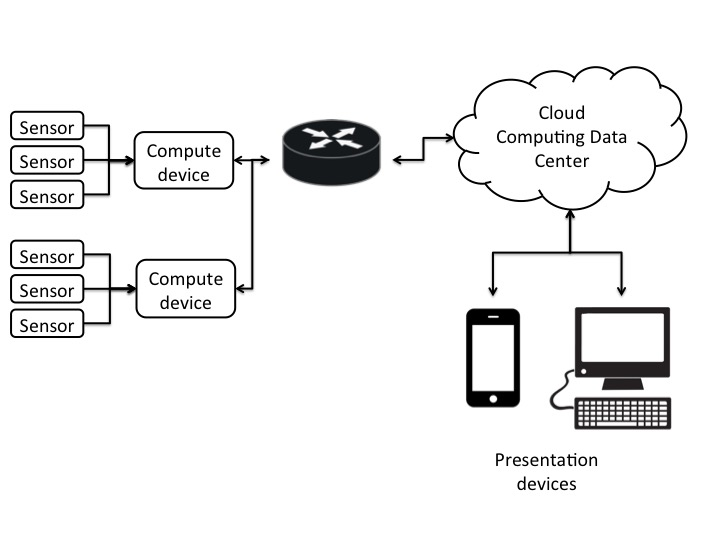
\includegraphics[width=0.75\textwidth]{images/IoT_diagram.jpg}
\caption{IoT full diagram }
\label{fig:1.1}
\end{figure}

Like many booming areas of technology, the internet of things revolution is
plagued by a lack of industry standards. As you can imagine there are thousands
of computing devices and sensors from different vendors that appear on the
market  every day , each one with his unique way to send  or store their data
in their centralized cloud computing centers.

Right now exist two main projects that are compiling to establish standards for
the IoT communications: 

\begin{itemize}
\item Open Interconnect Consortium (OIC): OIC is an industry group whose stated 
mission is to develop standards and certification for devices involved in the 
Internet of Things based around CoAP. OIC was created in July 2014 by Intel, 
Broadcom, and Samsung Electronics.\cite{OIC}

\item AllJoyn : AllJoyn is an open, universal, secure and programmable software 
connectivity and services framework that enables companies and enterprises to 
create inter-operable products that can discover, connect and interact directly 
with other AllJoyn-enabled products. \cite{AllJoyn}
\end{itemize}


Both standards try to solve a simple problem. Imagine you have smart light bulbs
in your house, all of them a device of your IoT network at home. What happened
if one them burns? You go and buy one but then you remember that all your
light bulbs at home are brand A and at the store there are only brand B
light bulbs. It should be possible to bring your any brand of light bulbs and
still work with the rest of the devices of your network. This will be possible
with communications standards among the industry.These two efforts are fighting
each other to generate these kind of standards in IoT communications. Which one
is the best ? maybe is too soon to have a winner, but in less than a decade
this question might be answered. 

In the meantime the Internet of Things revolution is here wetter we like it or
not. We live in houses with Computers insides our air conditions televisions
and cars; many of them connected to the internet. But as we have seen there are
parts that are being missing. Despite the efforts to develop standard network
protocols for IoT systems there is no effort to make the IoT systems analyze
their data among each others instead of send  all the data to Cloud Data centers
to be analyzed. This could be a problem in short future cause as we have seen
before the solution is not to add another server (specially when you have space
and economic constrains)


\section{Problem Definition}
\noindent

In order to understand the severity of the problem we have to understand the
magnitude of it, we have to understand that the rise of the internet of things
is real.  According to a study by the International Data Corporation (IDC)
\cite{IDC}, a market research analysis and advisory firm specialized in
information technology estimate the number of IoT devices is approaching  200
billion. And the number of sensors that track, monitor, or feed data to those
things is already more than 50 billion, with scientists talking about
trillion-sensor networks within 10 years. Of course, not all of those 200
billion things are actually wired and communicating on the Internet, but some
20 billion are. And, by 2020, this number will grow by 50\% to 30 billion
connected devices.\cite{EMC1}

But the rise of the internet of things means the rise of data. Imagine for a
moment that the 20 billion of devices try to send 1 Kilo Byte of data to the
centralized servers, this will create so much traffic that might be similar to
a security attack, collapsing the centralized data centers. One could imagine
that this is not a problem, that we might be exaggerating; but as we saw there
are actual problems like the one Virgin Atlantic airline has.

In 2014 the Boeing 787 aircraft ordered by Virgin Atlantic for delivery
dramatically increase the volume of data the airline will need to deal with
(half terabyte in a transatlantic flight). \cite{Finnegan} Because they can't
handle that much terabytes of data everyday coming from various airplanes they
are looking for cloud base solutions inside the airplanes. Now consider that
the space in an airplane is limited and expensive, moreover the electric
energy. A cloud base solution (adding servers inside the airplane) will require
both space and space and electric energy.

Besides that, the power consumption of these  IoT's Cloud Data Centers is a key
part to considerate. If current trends continue, a petaflop system will require 
100 megawatts to manage the IoT data \cite {Xizhou} (imagine that in an airplane)

The rise of IoT will lead to an explosion in the volume of data collected,
transmitted and processed.This will require novel and optimized solutions.  How
can we make the IoT networks self sustainable? Make them solve their own
compute problems without the need to send millions of data to the cloud data
centers?. How can we know when is really necessary to send the data to the cloud
data centers because the number of IoT systems is not efficient ( in terms of
energy and performance)? What kind of applications are good candidates for
these kind of solution? All these questions will be addressed in this work. 

\section{General Objective}
\noindent

The main objective is to find the maximum number of low ultra-low-voltage
microprocessors platforms that provides the maximum level of energy efficiency.

After finding this information for commons benchmarks it will be easy for the
industry of IoT systems to determine if their applications can take advantage
of communicate their IoT devices to process their own data instead of sending
the information to a data centers.

\section{Hypothesis}
\noindent

We are confident that with the current technology is possible to generate a
distributed system of of ultra-low-voltage microprocessors platforms (core
systems of the IoT devices). The part that we are concern is determine the
breaking point where is better to send the data to the cloud data centers. How
many systems is the maximum that these kind of network could support and still
being a good option in terms of energy efficiency?

In computing, performance per watt is a measure of the energy efficiency of a
particular computer architecture or computer hardware. Literally, it measures
the rate of computation that can be delivered by a computer for every watt of
power consumed.\cite{Burd} 


\begin{equation}
    Energy Efficiency = \dfrac {Performance}{Watts}
\end{equation}

We believe that the energy efficiency in an embedded cluster will have is the
behavior of the  figure~\ref{fig:1.2}. in the beginning the increment of the
number of nodes in our network will increment the performance (the top part of
the equation), but as the same time it increase the amount of watts will
increase making the energy efficiency flat at some point (if the lower part of
the equation increase the equation tends to decrease)


\begin{figure}[H]
\centering
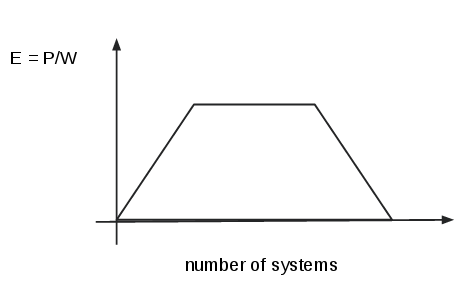
\includegraphics[width=0.75\textwidth]{images/graph_1.png}
\caption{Hypothesis of energy efficiency behavior in embedded cluster}
\label{fig:1.2}
\end{figure}

After finding these curves for command benchmarks it will be easy for the
industry of IoT systems to determine if their applications can take advantage
of communicate their IoT devices among each others instead of sending the
information to their data centers.


\section{Methodology}
\noindent

Recent researches \cite{Saldana} \cite{Gallego} \cite{McMahon} \cite{Liu} are 
showing an increasing interest in the topic.  All these research always talk
about the lack of three parts: 

\begin{itemize}
\item A low-voltage microprocessors platform with enough compute power
\item An operating system for Distributed System
\item A light communication protocol to distribute the workload among the
embedded platforms
\end{itemize}

The way we are going to address this will be:


\begin{itemize}

\item Chose the right embedded platform: There are dozens of embedded and IoT
platforms, this is why is necessary to make a deep analysis and choose the best
platform that feed our needs. (taking into consideration that sometimes the
systems might have heterogeneous platforms)

\item Chose the right communication and compute protocol: There are different
kinds of distributed compute protocols. Part of this investigation is to detect
the most reliable and suitable for our needs.

\item Chose the right Operating System for the system. Once we have selected
the appropriate embedded platforms, another variable in this investigation is
the number of Operating Systems. Either if is a micro kernel or a monolithic
kernel architecture there are more than a dozen of solutions to use.

\item Crate embedded clusters to measure energy efficiency. Once we have find
the best configuration (Hardware + Operating System + Communication Protocol )
in terms of energy efficiency , we can start to create a cluster of embedded
systems.

\item Release all the improvements and disagreements found Open Source and
public. All the improvements made into any technology (operating systems or
communication protocols) will be published with an open source license.

\item Implement solution on real application ( greenhouse ). In order to test
or hypothesis in a real application we will implement it on a real greenhouse.
Proving that the solution give an embedded system the power of reliability and
availability without the need of external and expensive servers 
\end{itemize}


\clearpage

	%Empieza configuracion de capitulo
\setstretch{1.0}
\titleformat{\chapter}[block]{\Large\bfseries}{CHAPTER \Huge\thechapter\vspace{25 pt}}{0 pt}{\\\fontsize{26}{36}\selectfont}
\titlespacing{\chapter}{0 pt}{30 pt}{50 pt}[0 pt]
\titleformat{\section}{\Large\bfseries}{\thesection}{0 pt}{\hspace{30 pt}}
\titleformat{\subsection}{\large\bfseries}{\thesubsection}{0 pt}{\hspace{30 pt}}
\pagestyle{fancy}
\fancyhead[LO,LE]{\footnotesize\textit{\leftmark}}
\fancyhead[RO,RE]{\thepage}
\fancyfoot[CO,CE]{}
%Termina configuracion de capitulo

\chapter{Objectives} %Cambia Marco Te'orico al nombre de tu capitulo
\setstretch{1.5} %Regresa el interlineado a 1.5

\normalsize

\section{General Objective}
\noindent

The main objective is to present a methodlogy to crate a self sustainable
network of ultra-low-voltage microprocessors platforms. It means the embedded 
devices interconected could process their own workload without the need of an 
external compute system

The purpose of this methodology is to give an experienced IoT  developer 
enough information to replicate the study. At the same time it offers the theoretical 
underpinning for understanding which method, set of methods, or so-called “best 
practices” can be applied an specific case


\section{Justification}
\noindent

The development of wireless sensor networks has reached a point where each 
individual node of a network may store and deliver a massive amount of 
(sensor-based) information at once or over time. Right now the total amount of 
user data (data payload) to be stored or processed doubles every two years. Consequently,
data will become a problem for traditional data aggregation strategies 
traffic-wise as well as with regard to energy efficiency. 

These problems start to be relevant in current industries. Such is the case of 
the Aircraft industry. On March of 2013 Virgin Atlantic was preparing for a 
significant increase in data as it embraces the internet of things, with a new fleet of highly 
connected planes each expected to create over half a terabyte of data per flight.

Speaking to the Computerworld UK magazine at the Economist Technology Frontiers 2103 event, Virgin 
Atlantic IT director David Bulman said that the airline company was expecting an 
"explosion" of information generated from a growing number of sources, from 
employees and customers to cargo containers and planes.

In particular, the introduction of Boeing 787 aircraft ordered by Virgin 
Atlantic for delivery in 2014  was expected to dramatically increase the volume 
of data the airline will need to deal with.

From the interview Bulman hightlight their current problems: 

\say{The challenge is what do you do with that amount of data when you are getting 
terabytes of data a day off your various airplanes? We are getting to the stage 
right now where we cannot deal with that much}

He added: 

\say{If you are talking that level of data you can't just chuck ten disks 
into your data centre anymore, you have to look at cloud based solutions and how 
you can store data.}

As we can see the lack of standard solutions for self sustainable networks is 
creating real problems among the industry


\clearpage

	%Empieza configuracion de capitulo
\setstretch{1.0}
\titleformat{\chapter}[block]{\Large\bfseries}{CHAPTER \Huge\thechapter\vspace{25 pt}}{0 pt}{\\\fontsize{26}{36}\selectfont}
\titlespacing{\chapter}{0 pt}{30 pt}{50 pt}[0 pt]
\titleformat{\section}{\Large\bfseries}{\thesection}{0 pt}{\hspace{30 pt}}
\titleformat{\subsection}{\large\bfseries}{\thesubsection}{0 pt}{\hspace{30 pt}}
\pagestyle{fancy}
\fancyhead[LO,LE]{\footnotesize\emph{\leftmark}}
\fancyhead[RO,RE]{\thepage}
\fancyfoot[CO,CE]{}
\setcounter{secnumdepth}{5}
%Termina configuracion de capitulo

\chapter{Theoretical Framework}
\setstretch{1.5} %Regresa el interlineado a 1.5

\normalsize
\noindent

This chapter will describe some basic topics to fully understand further
experiments and why we decided to do them. We will try to cover as much of the
topics needed to fully understand the problem and the proposed solution.
However will not cover deep topics as Operating Systems architecture nor
parallel programming concepts.


\section{The need of parallel computing}
\noindent

Based on all the current advantages we have today ( smart-phones, tablets,
smart cars and more ) thanks to the power the computer has achieve, one coudl
think that the computer design has been evolving like any other technology.
However the progress in the computer architectures has been much less
consistent.  During the first 25 years of electronic computers \footnote{since
1951 with the introduction of UNIVAC} the improvement in performance increase
about 25\% per year \cite{Hennessy}. 


It was until the late 1970s  when the world saw the emergence of the
microprocessor. This major change in technology aloud the industry to improve
the scalability of the integrated circuits. After the introduction of the
microprocessor the improvement in performance per year in the computer
architectures increase to 35\% \cite{Hennessy}   

But the advances in computer architecture were not the only one responsible for
this great increase in performance. In particular two significant changes make
the life of users easy. First, the elimination of assembly language with the
invention of the C programing language, a much more easy to read and use
programing language. The C programing language give the user the power to
handle memory and peripheral devices in a much more friendly way. Second, the
creation of standardized and free  operating systems, such as UNIX and its
clone, Linux. These operating systems lowered the cost and risk of bringing out
to the market brand new products

In the decade of 1980 the idea of making the microprocessor architecture faster
starts to take form with the RISC (Reduced Instruction Set Computer)
architecture .  The RISC microprocessor is designed to perform a smaller number
of types of computer instructions so that it can operate at a higher speed. 
The RISC-based computers raised the performance bar. This architecture
principle in conjunction with the transistor size reduction ( allowing to have
much more compute power in less space) led to 16 years of sustained growth in
performance at an annual rate of over 50i\%

It was around the years 2003 to 2005 that a dramatic change seized the
semiconductor industry and the manufactures of processors. The increasing of
computing performance in processors, based on simply screwing up the clock
frequency, could not longer be sustainable. The problem with increasing the
frequency in the microprocessor is that the heat in the chip also increase.  In
fact in 2004 Intel canceled its high-performance projects declaring that
\textit{the road to higher performance would be via multiple processors per
chip rather than via faster uniprocessors}

The answer of the industry to that development, in order to still meet Moore's
law \footnote{the number of transistors in a dense integrated circuit doubles
approximately every two years.}, was the shifting to real parallelism by
doubling the number of processors on one chip die. This was the birth of the
multi-core area. 

With the multi core are there was a need to change the paradigm in programing
languages. The programs that had been designed before this change were mostly a
sequence of instructions to calculate or control a system. With the multi core
architecture came the birth of the parallel programing. The parallel programing
codes are properly designed to take advantage of parallelism can execute faster 

However not all the problems can be solved using parallel programing
techniques. In order to use this approach the problem need to be represented as
a collection of simultaneously executing tasks. This is especially the case in
many areas of scientific, mathematical, and artificial intelligence
programming. After the birth of the parallel computing all these technology
areas had a growth never seen before

At the same time that the parallel computing came many other technologies was
already established: the emergence of the Internet and the World Wide Web, the
popularity of cell-phones since 2000 and the broadly use of laptops. According
to \cite{Hennessy} all  these technologies have led to three different computing
markets: desktop computing, servers and embedded. 

The problem we have will require a deep understanding of the server and
embedded components. So far we have seen why the world needed the parallel
computing as well as the evolution of the computer architecture that aloud us
to arrive here.

\section{Servers Systems}
\noindent

The growth of mobile personal computers coupled with the popularity of
cellphones changed the role of servers to provide scale and reliable storage
and computing services. The emerge of faster Internet connections accelerate
the demand of web-based services make the transition of compute power from
personal computers to servers

But the fact of provide storage and compute services to thousands of users came
with a lot of responsibility. A failure of server systems is far more
catastrophic than failure of a single desktop, since these servers must operate
seven days a week, 24 hours a day Is because of this that reliability is a key
factor for a server system.

A second key feature of server systems is scalability. With the number of users
changing every minute the ability to scale up the computing capacity
in server is crucial. A web sale page should be able to response every as well
as during a peak hour for Christmas shoppings.

The third key feature is throughput. Servers are designed for efficient
throughput \footnote{Throughput is a measure of how many units of information a
system can process in a given amount of time} in terms of transactions per
minute or Web pages served per second. From the user perspective point of view
is the speed of response.

Is because of these three factors that the server technology has change. The
cloud era is dominating the computing and storage services.  According to \cite
{Farhan} \textit{"Cloud computing is set of resources and services offered
through the Internet"}. Cloud services are delivered from data centers located
around the world.  Cloud computing provides virtual resources via internet. The
best example of cloud computing is the streaming video services. Nowadays users
can stream online videos  at any time, without the need to storage the movie at
home. All the resources and infrastructure are provided upon request. With this
the scalability, reliability and manageability are guaranteed by the compute
service providers. 

\section{Embedded Systems}
\noindent

The birth of multi core architecture not only provide the servers with much
more compute power it also break the paradigm of use low compute power
microprocessors for embedded platforms. Now it was possible to have more
compute power with less frequency. Thanks to this radical change there has been
a rapid evolution of the compute and multimedia capabilities of embedded
systems. At the point where have more computer power in our cellphones than all
of NASA back in 1969 \cite{Michio}

According to \cite{Hallinan} \textit{"An embedded system is a special-purpose
system in which the computer is completely encapsulated by the device it
controls"} Unlike a general-purpose computer, such as a personal computer, an
embedded system performs pre-defined tasks, usually with very specific
requirements. Examples of these are:microwaves, washing machines, printers, and
GPS (Global Positioning System) systems. All those electronic gadgets that
started to emerge 15 years ago \cite{Nur}.

The variety of the embedded applications requires at the widest spread
of processing power and cost. They include 8-bit and 16-bit processors that may
cost few cents, 32-bit microprocessors that execute 100 million instructions
per second and cost less than few dollars, and high-end processors for the
newest video games or network switches that cost at least 100 dollars and can
execute a billion instructions per second.\cite{Hennessy}

Since its origins, the RISC technology has been the default technology in the
more complex embedded architectures. Due to the fact that The RISC
microprocessor is designed to perform a smaller number of types of computer
instructions the power consumption can be much more lower. This architecture
concept was fine until the new embedded applications such as smart-phones,
tablets and smart TVs start to appear.

The increment in the complexity of the new embedded applications started to
require more specialized integrated circuits that could help the microprocessor
with all these task in parallel . Wireless networking cards, Digital Signal
Processors, I/O controls, peripherals ( such as USB controllers ) and analog
interfaces (including ADCs and DACs) became part of the requirements of an
embedded platform. Soon the architecture designers realize that the
communication with all these components decrease the performance and increase
the power consumption. Is because of this that the last decade saw the emerge
of the System of a Chip (SOC)  embedded platforms. 

The SoC is an integrated circuit with all these components into a single chip.
With all these components in the same integrated circuit the communication
latency and power consumption was reduced considerably. Since the birth of the
SoC architecture the variety of gadgets using embedded platforms has increasing
every year.  Every year some basic goals are pursued:  increment in compute
performance, cost,  size and power density reduction.

\section{Embedded Linux Systems}

Computers are everywhere, we already know that computers aren't just on our
desktops, they are in our kitchens  and increasingly in our living rooms
holding our music collections. They're also in our microwave ovens, our regular
ovens, our cellphones, and our portable digital music players.

Until not too long time ago, embedded systems were not very powerful, and they
ran special-purpose, proprietary operating systems that were very different
from industry-standard ones. (Plus, they were much harder to develop for.)
Today, embedded computers are as powerful as, if not more than, a modern home
computer. (Consider the high-end gaming consoles, for example.)

Along with this power comes the capability to run a full-fledged operating
system such as Linux. Using a system such as Linux for an embedded product
makes a lot of sense. It was thanks to the free operating system UNIX and its
easy user experience, that the number of users of computer increase in the
early birth of personal computers. The evolution of UNIX, Linux, has been one
of the most sustainable projects in the history of computing. The fact that a
large community of developers find novel ways to improve performance and fix
critical failures every day are the key to think that Linux could be the best
solution in terms of sustainability for embedded platforms.

According to \cite{Hallinan} there are multiple reasons why Linux is the best choise
for current embedded platforms 

\begin{enumerate}
\item Linux supports a huge variety of applications and networking protocols.
Linux is scalable, from small consumer-oriented devices to large, heavy-iron,
carrier-class switches and routers.
\item Linux can be deployed without the royalties required by traditional proprietary
embedded operating systems.
\item Linux has attracted a huge number of active developers, enabling rapid support
of new hardware architectures, platforms, and devices.
\item An increasing number of hardware and software vendors, including virtually all
the top-tier manufacturers and ISVs, now support Linux.
\end{enumerate}

For these and other reasons, we are seeing an accelerated adoption rate of
Linux in many common embedded platforms. With the birth of the SoC systems the
use of these complete operating systems was necessary due to the need of handle
process concurrency, memory management and network connectivity.

Although the idea of using Linux as main operating system for embedded platform
was easy in reality it was not. With too many configure options and no standard
methodologies or templates to reuse the process to customize a Linux Operating
System for embedded platforms became a complex work for software engineers.
Every new embedded company create his own version ( according to his needs
without any standards) with very low maintainability and robustness. In 2010
there was a change in the industry of embedded systems, the announce of a
project to solve these kind of problems: The Yocto project.

The Yocto Project is an open source collaboration project that provides
templates, tools and methods to help you create custom Linux-based systems for
embedded products regardless of the hardware architecture\cite{yocto-project}.
It was founded in 2010 as a collaboration among many hardware manufacturers,
open-source operating systems vendors, and electronics companies to bring some
order to the chaos of embedded Linux development.\cite{Leppakoski}

The Yocto project  is a  complete embedded Linux development environment with
tools, meta-data, and documentation. The free tools are easy to get started
with, powerful to work with (including emulation environments, debuggers, an
Application Toolkit Generator, etc.) and they allow projects to be carried
forward over time without causing you to loose optimizations and investments
made during the project's prototype phase. The Yocto Project fosters community
adoption of this open source technology allowing its users to focus on their
specific product features and development.

The Yocto Project through the Poky build tool provides an open source
development environment (figure~\ref{fig:3.1})  targeting the ARM, MIPS,
Power-PC and x86 architectures for a variety of platforms including x86-64 and
emulated ones.  You can use components from the Yocto Project to design,
develop, build, debug, simulate, and test the complete software stack using
Linux, the X Window System, GNOME Mobile-based application frameworks, and Qt
frameworks. 

\begin{figure}[H]
\centering
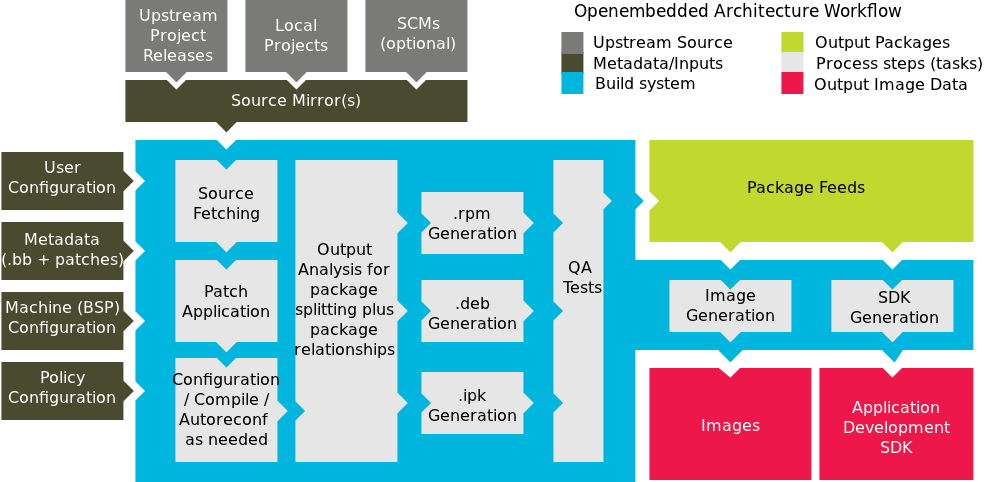
\includegraphics[width=0.75\textwidth]{images/yocto-environment.png}
\caption{The Yocto project development environment}
\label{fig:3.2}
\end{figure}

As we can see the Yocto project will play an important role in the IoT world.
If we want to develop a solution standard for multiple platforms we might adapt
it for the Yocto project. If we do this our solution will be deployable into
multiple IoT devices due to the bast amount of platforms ( sensors and
processing devices ) that use the Yocto project everyday.

\section{Ubiquitous Computing and IoT}
\noindent

The combination of all these factors (the cost, size, and power density
reduction) in combination with the increase in computing power and connectivity
has caused the computing technology to evolve into ubiquitous computing.
According to Mark \cite{Mark}, ubiquitous computing is \textit{"the method of
enhancing computer use by making many computers available throughout the
physical environment, but making them effectively invisible to the user"}. This
mean that the computing power is available anywhere and at any time


According to \cite{Nur} currently we are moving from ubiquitous computing into
advanced ubiquitous computing. An advanced ubiquitous computing is an extension
of ubiquitous environment that improve connectivity between devices. The major
characteristics of this environment can be stated as follows: 

\begin{itemize}
\item Large number of heterogeneous devices
\item New communication technology
\end{itemize}

This  devices include devices such as notebook computers, tablets, smartphones
and wearable computers. Most of these devices operate under many different
operating systems. New communication technology 4G , 5G and the introduction of
IPv6 provides bigger and faster of data bandwidth and much better than 3G in
data performance.

One of the most accurate definitions of the IoT is the one given by
\cite{Bahga} where it mentions that "Internet of Things refers to physical and
virtual objects that have unique identities and are connected to the internet
to facilitate intelligent applications [...] smarter". The IoT enables the
interconnection via the Internet of computing devices embedded in everyday
objects, enabling them to send and receive data. As you can see the differences
with traditional embedded systems are the internet connectivity and less power
consumption.  IoT systems must always be connected to the internet which
require a lower power consumption

The IoT computing is new era of computing technology that we have to explore.In
collaboration with the cloud computing the capability to have smart
applications in multiple scenarios is imminent. In the middle of all these
technology an invisible architecture design was established , transparent for
the user , but always there sustaining the reliability, scalability and
reliability of the systems, it was the distributed architecture systems.

\section{Distributed Systems}
\noindent

We define a distributed system as one in which hardware or software components
located at networked computers communicate and coordinate their actions only by
passing messages. This simple definition covers the entire range of systems in
which networked computers can usefully be deployed.

Computers that are connected by a network may be spatially separated by any
distance. They may be on separate continents, in the same building or in the
same room. Our definition of distributed systems has the following significant
consequences:


\begin{enumerate}

\item \textbf{Concurrency:}
In a network of computers, concurrent program execution is the norm. I can
do my work on my computer while you do your work on yours, sharing resources
such as web pages or files when necessary. The capacity of the system to handle
shared resources can be increased by adding more resources (for example.
computers) to the network.

\item \textbf{No global clock:}
When programs need to cooperate they coordinate their actions
by exchanging messages. Close coordination often depends on a shared idea of
the time at which the programs actions occur. But it turns out that there are
limits to the accuracy with which the computers in a network can synchronize
their clocks there is no single global notion of the correct time. This is a
direct consequence of the fact that the only communication is by sending
messages through a network.

\item \textbf{Independent failures:}
All computer systems can fail, and it is the
responsibility of system designers to plan for the consequences of possible
failures. Distributed systems can fail in new ways. Faults in the network
result in the isolation of the computers that are connected to it, but that
doesn't mean that they stop running. In fact, the programs on them may not be
able to detect whether the network has failed or has become unusually slow.
Similarly, the failure of a computer, or the unexpected termination of a
program somewhere in the system (a crash), is not immediately made known to the
other components with which it communicates. Each component of the system can
fail independently, leaving the others still running.

\end{enumerate}


Each one these characteristics is also present in a modern IoT system. As we can
see in (figure~\ref{fig:3.1}). As we can see these three characteristics of a
distributed system are also present in an IoT system. 

\begin{figure}[H]
\centering
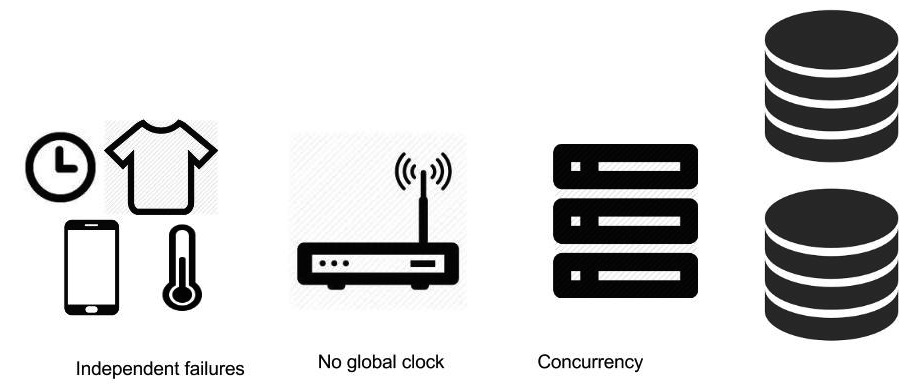
\includegraphics[width=0.75\textwidth]{images/IoT_distributed.jpg}
\caption{IoT system as a distributed system}
\label{fig:3.1}
\end{figure}


\begin{enumerate}
\item \textbf{Concurrency}
In an IoT system there are multiple systems trying to use the same resource.
For example all the IoT devices are trying to access the same data base or the
even the same access's point. All of them are fighting for similar resources , a
good IoT design need to schedule the use of the limited resources in an efficient
way.

\item \textbf{No global clock}
None of the systems in an IoT network (either sensors or processing devices)
have the same clock. They have to use a message base mechanism to communicate
each other. 

\item \textbf{Independent failures}
In a regular IoT network multiple systems could fail (either sensors,
processing devices or one of the data centers) and despite of that all the
others should keep working without any problem. 

All these characteristics enforce the idea that the nature of an IoT system is
being treated as a distributed system. With this main idea is much more simple
to adapt the solutions of the distributed systems into our embedded distributed
system.

\end{enumerate}

\section{Message-Passing Interface Library}
\noindent

The Message-Passing Interface (MPI) is a message-passing library interface
specification. MPI addresses primarily the message-passing parallel programming
model, in which data is moved from the address space of one process to that of
another process through cooperative operations on each process

MPI is not a language, and all MPI operations are expressed as functions,
subroutines, or methods, according to the appropriate language bindings which,
for C and FORTRAN, are part of the MPI standard. The standard has been defined
through an open process by a community of parallel computing vendors, computer
scientists, and application developers

Despite all the advantages that MPI has it is not widely used in embedded
systems (due to the fact that these abstraction layers require extensive
system resources with comprehensive operating systems support, which may not be
available to an embedded platform) but as we have seen this is now possible. We
do have a powerful ultra-low-voltage microprocessor platform
\cite{minnowboard} and we do have robust distributed operating systems running on
those platforms. The missing part now is to set up the message passing library
interface on the top of all the system. 

Recent researches \cite{Saldana} \cite{Gallego} \cite{McMahon} describe
proof-of-concept MPI implementations targeting embedded systems, showing an
increasing interest in the topic. However none of theme has been implemented in
the current embedded Linux operating systems (like the ones generated with
Yocto project\cite{yocto-project}) nor the standard Linux (like
Fedora\cite{fedora})

After a quick review on the current operating systems we found that the only
one missing the MPI implementation was actually the Yocto project.


\begin{center}
\begin{tabular}{ | l | r |}
    \hline
    Operating System & MPI library  \\ \hline
    Fedoras & Implemented  \\ \hline
    Clear Linux for Intel Architecture & Implemented  \\ \hline
    OS generated with Yocto project & Not Implemented  \\ \hline
\end{tabular}
\captionof{table}{Linux OS supported MPI implementation on MinnowBoard MAX}
\label{tab:4.2}
\end{center}


\section{Performance and Power Efficiency}

\noindent

The meaning of performance may be different according to the application.
The user of a desktop computer may say a computer is faster when a program runs in less
time, while an Amazon.com administrator may say a computer is faster when it
completes more transactions per hour. The computer user is interested in 
reducing response time (the time between the start and the completion of an 
event) \cite{Hennessy} also referred to as execution time. The administrator of a large data 
processing center may be interested in increasing throughput (the total amount 
of work done in a given time.) \cite{Hennessy}. 

According to \cite{Hennessy} in comparing design alternatives, we often want to
relate the performance of two different computers, say, X and Y. The phrase ''X
is faster than Y'' is used here to mean that the response time or execution
time is lower on X than on Y for the given task. In particular, ''X is n times
faster than ''  will mean \ref{eq:2}:

\begin{equation}\label{eq:2}
n = \frac{Execution time x}{Execution time y}
\end{equation}

Since execution time is the reciprocal of performance, the following
relationship holds in formula \ref{eq:3}:

\begin{equation}\label{eq:3}
n = \frac{Execution time x}{Execution time y} = \frac{\frac{1}{Performance
x}}{\frac{1}{Performance y}} = \frac{Performnace x}{Performance y}
\end{equation}

Another metric to considerate is the throughput. According to \cite{Hennessy}
\textit{"the throughput of X is 1.3 times higher than Y signifies that the
number of tasks completed per unit time on computer X is 1.3 times the number
completed on Y"} . Unfortunately, time is not always the metric quoted in
comparing the performance of computers. The only consistent and reliable
measure of performance is the execution time of real programs. 

The most straightforward definition of execution time is given by
\cite{Hennessy} \textit{"it is called wall-clock time, response time, or elapsed
time, which is the latency to complete a task, including disk accesses, memory
accesses, input/output activities, operating system over head everything"}.
Even in current multi processors world this is transparent for the users,  the
response time seen by the user is the elapsed time of the program, not the CPU
time.

But in parallel programing the performance metric is measure in a different
way.  With the current compute power of compute devices is possible to create a
cluster of computers. All of the inter-connected in a network that provides the
maximum level of performance with the less amount of power consumption. This
characteristic is determined by the power efficiency of the network. The power
efficiency is quantified by performance per watt \cite{Jun}

The critical part is to determine the breaking point where is better to send
the data to the cloud data centers. How many systems is the maximum that these
kind of network could support and still being a good option in terms of energy
efficiency

The development of metrics to evaluate energy efficiency on the basis of
performance and power models is described in \cite{Dong}. According to
\cite{Dong} the formula for computing the theoretical maximum speedup (or
performance) achievable through parallelization is \ref{eq:4}

\begin{equation}\label{eq:4}
Perf = \frac{1}{(1 - f) + \frac{f}{n}}
\end{equation}

Where \textit{n} is the number of processors,  \textit{f} is the fraction of
computation that programmers can parallelize  ( form 0 to 1 ) . To model the
power consumption for a \textit{P} many-core processor, \cite{Dong} introduce a
new variable, \textit{k}, to represent the fraction of power the processor
consumes in idle state \ref{eq:5}. 

\begin{equation}\label{eq:5}
\frac{Perf}{W} = \frac{1}{(1 + (n -1 ) k (1 - f))}
\end{equation}

In \cite{Dong} their analysis clearly demonstrates that a symmetric many-core
processor can easily  lose its energy efficiency as the number of cores
increases. To achieve the  best possible energy efficiency, their  work
suggests a many-core alternative, featuring many small, energy-efficient cores
integrated with a full-blown processor. They also show that by knowing the
amount of parallelism available in an application prior to execution, is
possible to  find the optimal number of active cores for maximizing performance
for a given cooling capacity and energy in a system

\section{Benchmarks}

In computer science a benchmark is a test to measure the performance of
multiple applications over the same standard way. The best choice of benchmarks
to measure performance are real applications. Due to the complexity of the
current applications the software engineers are making small versions of them
to be used as benchmarks. According to \cite{Hennessy} there are three kind of
them: 

\begin{itemize}
\item kernels, which are small, key pieces of real applications.
\item Toy programs, which are 100-line programs from beginning programming
assignments.
\item Synthetic benchmarks, which are fake programs invented to try to match the
profile and behavior of real applications.
\end{itemize}

One of the most successful attempts to create standardized benchmark
application suites has been the SPEC (Standard Performance Evaluation
Corporation), which had its roots in the late 1980s efforts to deliver better
benchmarks for workstations\cite{Hennessy}. All the SPEC benchmark suites and
their results are found at www.spec.org.

In terms of parallel and distributed computing (MPI) there are already numerous
MPI benchmark suites available , such as Mpptest \cite{Gropp}, MP-Bench
\cite{Calderon} and  SKaMPI \cite{Hoefler} are examples of them. Many of give
timing results for message passing routines. This is useful for performance
modelling and analysis of parallel programs, as well as for understanding the
performance of parallel machines. Based on the results in \cite{Grove} we
decided to use MPIbench as our default benchmark testing framework. MPIbench is
a benchmark that allows to evaluate the performance of MPI on MPP's and cluster
of workstations. MPIbench tests different MPI calls.

\subsection{MPIbench}
\noindent

The benchmarks we are going to run are the MPIbench (or MPbench) version 4
\cite{mpibench}.This is a program to measure the performance of some critical
MPI functions. By critical we mean that the behavior of these functions can
dominate the run time of a distributed application.

MPIBench currently tests eight different MPI calls. The following functions are
measured:

\begin{itemize}
    \item Bandwidth (BB/second)
    \item Gap Time (time to launch a message and continue) (Us)
    \item Roundtrip or 2 * Latency (transactions/second)
    \item Asynchronous Bidirectional bandwidth (KB/second)
    \item Broadcast (KB/second)
    \item Sum reduction (KB/second)
    \item All-reduce (KB/second)
    \item AlltoAll (KB/second)
\end{itemize}



All tests are timed in the following manner.

\begin{itemize}
    \item Set up the test.
    \item Start the timer.
    \item Loop of operations over the message size as a power of two and the
iteration count.
    \item Verify that those operations have completed.
    \item Stop the timer.
    \item Compute the appropriate metric
\end{itemize}

By default, MPIBench measures messages from 4 bytes to 216 bytes, in powers of
two for 100 iterations. Each test is run a single time before testing to allow
for cache setup and routing. The cache is then flushed before each repetition
and before each new message size is tested. The cache is not flushed however
between iterations on the same message size, which are averaged

We will describe each one of the tests in order to understand the experiments.


\subsubsection{Bandwidth}

MPIBench measures bandwidth with a doubly nested loop. The outer loop varies the
message size, and the inner loop measures the send operation over the
iteration count. After the iteration count is reached, the slave process
acknowledges the data it has received by sending a four byte message back to
the master. The master's pseudo code for this test is as follows:

\begin{minipage}{\textwidth}
\end{minipage}

\begin{minipage}{\linewidth}
\begin{lstlisting}[frame=single,numbers=left]
do over all message sizes 
    start timer
    do over iteration count 
        send(message size) 
        recv (4)
    stop timer
\end{lstlisting}
\end{minipage}

The slaves' pseudo code is as follows:

\begin{minipage}{\textwidth}
\end{minipage}

\begin{minipage}{\textwidth}
\begin{lstlisting}[frame=single,numbers=left]
do over all message sizes 
    start timer
    do over iteration count 
        recv(message size) 
        send(4)
    stop timer
\end{lstlisting}
 \end{minipage}

\subsubsection{Bidirectional Bandwidth}

MPIBench measures bidirectional bandwidth with a doubly nested loop. The outer
loop varies the message size, and the inner loop measures the send operation
over the iteration count. Both processes execute a non-blocking receive, then a
non-blocking send, and then a wait for each iteration. The next iteration is
prevented from proceeding until the previous one is finished by the MPLWaitall0
call, which will not allow execution to continue until both messages have been
completed.

The code for this test is as follows:
 
\begin{minipage}{\textwidth}
\end{minipage}

\begin{minipage}{\textwidth}
\begin{lstlisting}[frame=single,numbers=left]
 do over all message sizes
    start timer
    do over iteration count
        immediate (nonblocking) receive(message size)
        immediate (nonblocking) send(message size)
        wait until messages on both ends have been received
    stop timer
\end{lstlisting}
\end{minipage}

\subsubsection{Roundtrip}

Roundtrip times are measured in much the same way as bandwidth, except that,
the slave process, after receiving the message, echoes it back to the master.
This benchmark is often referred to as ping-pong. Here our metric is
transactions per second, which is a common metric for database and server
applications. No acknowledgment is needed with this test as it is implicit
given its semantics.

The master's pseudo code for this test is as follows:

\begin{minipage}{\textwidth}
\end{minipage}

\begin{minipage}{\textwidth}
\begin{lstlisting}[frame=single,numbers=left]
  do over all message sizes 
    start timer
    do over iteration count
        send(message size)
        recv(message size) 
        stop timer
\end{lstlisting}
\end{minipage}

The slaves' pseudo code is as follows:

\begin{minipage}{\textwidth}
\end{minipage}

\begin{minipage}{\textwidth}
\begin{lstlisting}[frame=single,numbers=left]
do over all message sizes 
    start timer
    do over iteration count
        recv(message size)
        send(message size)
    stop timer
\end{lstlisting}
\end{minipage}

\subsubsection{Application Latency}

Application latency is something relatively unique to MPBench. This benchmark
can properly be described as one that measures the time for an application
to issue a send and continue computing. This benchmark is the same as
bandwidth except that we do not acknowledge the data and we report our
results in units of time.

The master's pseudo code for this test is as follows:

\begin{minipage}{\textwidth}
\end{minipage}

\begin{minipage}{\textwidth}
\begin{lstlisting}[frame=single,numbers=left]
do over all message sizes 
    start timer
    do over iteration count 
        send(message size) 
    stop timer
\end{lstlisting}    
\end{minipage}

The slaves' pseudo code is as follows:

\begin{minipage}{\textwidth}
\end{minipage}

\begin{minipage}{\textwidth}
\begin{lstlisting}[frame=single,numbers=left]
   do over all message sizes 
        start timer
        do over iteration count 
            recv(message size) 
        stop timer
\end{lstlisting}
\end{minipage}

\subsubsection{Broadcast and Reduce}

Both of these benchmarks return the number of megabytes per second computed
from the iteration count and the length argument given to function call.

Here is the pseudo code for both the master and the slave:

\begin{minipage}{\textwidth}
\end{minipage}

\begin{minipage}{\textwidth}
\begin{lstlisting}[frame=single,numbers=left]
   do over all message sizes 
        start timer
        do over iteration count
            reduce or broadcast(message size)
        stop timer
\end{lstlisting}
\end{minipage}

\subsubsection{AllReduce}

AllReduce is a derivative of an all-to-all communication, where every
process has data for every other. While this operation could easily be
implemented with a reduce followed by a broadcast, that would be highly
inefficient for large message sizes. 

Here is the pseudo code for both the master and the slave:

\begin{minipage}{\textwidth}
\end{minipage}

\begin{minipage}{\textwidth}
\begin{lstlisting}[frame=single,numbers=left]
    do over all message sizes 
        start timer
        do over iteration count 
            allreduce(message size) 
        stop timer
\end{lstlisting}
\end{minipage}

\subsubsection{All-to-all}

MPBench measures a kind of round-robin communication among multiple
processes. The outer loop varies the message size, and the inner loop
measures the send operation over the iteration count. Each process sends a
message of the size of the total message size divided by the number of
processes to every other process.

The code for this test is as follows:

\begin{minipage}{\textwidth}
\end{minipage}

\begin{minipage}{\textwidth}
\begin{lstlisting}[frame=single,numbers=left]
    do over all message sizes 
        start timer
        do over iteration count 
            all-to-all(message size)
        stop timer
\end{lstlisting}
\end{minipage}

\clearpage

	%Empieza configuracion de capitulo
\setstretch{1.0}
\titleformat{\chapter}[block]{\Large\bfseries}{CAP'ITULO \Huge\thechapter\vspace{25 pt}}{0 pt}{\\\fontsize{26}{36}\selectfont}
\titlespacing{\chapter}{0 pt}{30 pt}{50 pt}[0 pt]
\titleformat{\section}{\Large\bfseries}{\thesection}{0 pt}{\hspace{30 pt}}
\titleformat{\subsection}{\large\bfseries}{\thesubsection}{0 pt}{\hspace{30 pt}}
\pagestyle{fancy}
\fancyhead[LO,LE]{\footnotesize\emph{\leftmark}}
\fancyhead[RO,RE]{\thepage}
\fancyfoot[CO,CE]{}
%Termina configuracion de capitulo

\chapter{Reglas de Presentaci'on} %Cambia al nombre de tu capitulo
\setstretch{1.5} %Regresa el interlineado a 1.5

\normalsize
\noindent
Este manual de tesis se basa, en parte, del estilo establecido por la Rector'ia de la Universidad Virtual (UV) del Sistema Tecnol'ogico de Monterrey \cite{Demo:manualUV} y publicado por la American Psychological Association (APA) \cite{Demo:APA,Demo:manualAPA}. Los alumnos de las maestr'ias de la EGIA (Escuela de Graduados en Ingenier'ia y Arquitectura) del ITESM Campus Guadalajara deben considerar que es imprescindible apegarse a las reglas de estilo que se presentan en este manual.

Las siguientes reglas de formato son aplicables a las maestr'ias ofrecidas por la EGIA. Aseg'urate de seguirlas minuciosamente. Este manual est'a escrito estrictamente de acuerdo a las reglas generales y particulares que se mencionan a continuaci'on, as'i que le sirve como modelo para escribir tanto su documento de anteproyecto de tesis, como su documento final.

\section{Reglas generales}
\noindent
\begin{enumerate}
	\item Imprime solamente en un lado de la p'agina.
	\item Usa sangr'ias para cada p'arrafo nuevo, a excepci'on del primer p'arrafo que sigue a un cap'itulo, secci'on o subsecci'on.
	\item Inicia cada cap'itulo en una p'agina nueva.
	\item No dejes l'ineas aisladas al inicio de una p'agina. Escribe por lo menos un p'arrafo en su parte superior de al menos cuatro l'ineas.
	\item Utilizar una p'agina nueva para las referencias bibliogr'aficas como se muestra en este manual.
	\item Separa las s'ilabas siguiendo estrictamente las reglas gramaticales.
	\item Los trabajos producidos en impresoras de puntos son inaceptables, as'i como aqu'ellos producidos en otros medios que no aseguren una alta calidad de impresi'on. Se recomienda utilizar impresoras del tipo postscript.
	\item Centra los t'itulos de las p'aginas preliminares y la bibliograf'ia. Por ejemplo: Dedicatoria, Agradecimientos, Resumen, Contenido, Lista de Tablas y figuras y Bibliograf'ia (ver como ejemplo las p'aginas preliminares de este manual).
	\item Los cap'itulos del cuerpo del documento deben estar justificados a la izquierda y escritas en negritas. El t'itulo del cap'itulo correspondiente lleva may'usculas al inicio de todas las palabras, a excepci'on de las palabras cortas como: de, un, una, el, la, etc. Por ejemplo: \textbf{Dise'no de una Plataforma de Decodificaci'on}.
	\item Las subdivisiones de los cap'itulos deben estar escritas en negritas y min'usculas a excepci'on de la primera letra de la oraci'on.
	\item La silustraciones y tablas podr'an ser presentadas horizontalmente si no caben de manera vertical.
\end{enumerate}

\section{Tipo de letra}
\noindent
\begin{enumerate}
	\item Si emplea el procesador de textos Word\copyright  de Microsoft\textsuperscript{\texttrademark} o alguno similar, utilice letra de tipo Times New Roman de tama'no 12 puntos para la redacci'on del documento. Si usted escribe el documento en \LaTeX, utilice el layout disponible para tal efecto. No use letra cursiva excepto para las palabras cuyo origen sea de un idioma diferente al Espa'nol.
	\item Usa el mismo tipo de letra para todo el manuscrito; incluyendo las p'aginas preliminares, las referencias bibliogr'aficas y los anexos.
	\item Podr'as usar tama'nos reducidos de letras solamente en los pies de p'agina, pies de ilustraciones y tablas y citas textuales de otros trabajos.
	\item Usa el mismo tipo de letra para numerar ilustraciones y tablas, el cual puede ser diferente del tipo de letra usado para el texto del trabajo\footnote{De preferencia utilizar todas las especificaciones de este manual. En caso de utilizar, por ejemplo, el editor de texto Word ajustar las caracter'isticas del mismo para que cumplan con todas las especificaciones.\label{footnote}}.
	\item Usa numeraci'on ar'abiga (1, 2, 3, etc.) en la numeraci'on de secciones, subsecciones y en los n'umeros de p'agina. No se permiten cursivas para estos n'umeros.
\end{enumerate}

\section{Ecuaciones}
\noindent
\begin{enumerate}
	\item La presentaci'on de las ecuaciones deber'a realizarse con el uso de un editor de ecuaciones.
	\item Puedes utilizar un estilo de letra diferente al del texto para las ecuaciones.
	\item Puedes numerar las ecuaciones a trav'es del escrito si lo consideras pertinente. Si es as'i, poner la numeraci'on justificada a la derecha de las ecuaciones. Ejemplo:
\end{enumerate}

Si consideramos una transmisi'on de s'imbolos sobre un canal con modulaci'on BPSK (\emph{Binary Phase Shift Keying}) no codificada, y utilizamos una demodulaci'on coherente\footnote{El demodulador conoce la frecuencia y la fase de la onda recibida.\label{footnote}}, la probabilidad de error \begin{math}P_b(e)\end{math} sobre un canal gaussiano se puede expresar bajo la forma [7]:
\[P_b(e)=Q\left(\sqrt{\frac{2E_b}{N_0}}\right)\]
donde \begin{math}Q(.)\end{math} es la funci'on de error de una variable aleatoria gaussiana normalizada:
\[Q(x)=\int_x^\infty \frac{1}{\sqrt{2\pi}}e^{-\frac{u^2}{2}}du\]
El l'imite de la capacidad de informaci'on cuando \begin{math}R \to 0\end{math} es derivado de la ecuaci'on \begin{math}\lim_{R \to 0} [1-H_b(e)]=\frac{E_b}{(ln 2) N_0}\end{math}. Re-escribi'endolo, obtenemos:
\[
\begin{aligned}
\frac{E_b}{N_0}&=ln 2(1-H_b(e))\\
&=ln 2(1+P_b(e)log_2P_b(e)+(1-P_b(e))log_2(1-P_b(e)))
\end{aligned}
\]

\section{Figuras}
\noindent
\begin{figure}[H]
\centering
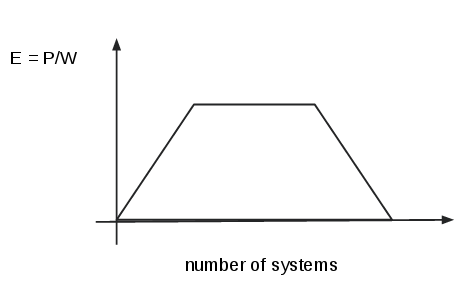
\includegraphics[width=0.75\textwidth]{images/graph_1.png}
\caption{Hypothesis of energy efficiency behaivor in embedded cluster}
\label{fig:4.1}
\end{figure}

\begin{figure}[H]
\centering
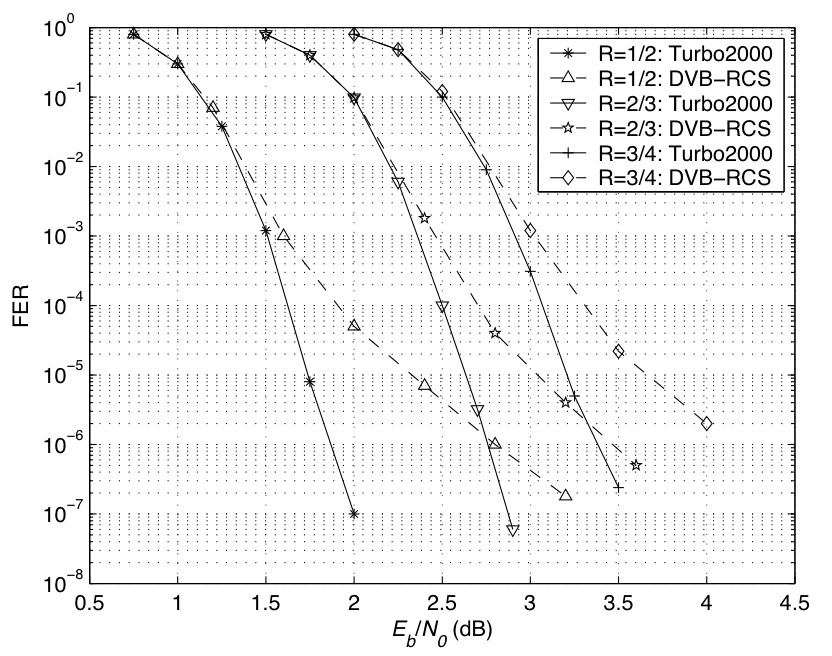
\includegraphics[width=0.7\textwidth]{images/figura4_2}
\caption{Comparaci'on del desempe'no de FER entre Turbo2000 y DVB-RCS. Par'ametros de la simulaci'on: Tama'no = 188 bytes, 8 iteraciones, q=4, QPSK y AWGN.}
\label{fig:4.2}
\end{figure}

\begin{figure}[H]
\centering
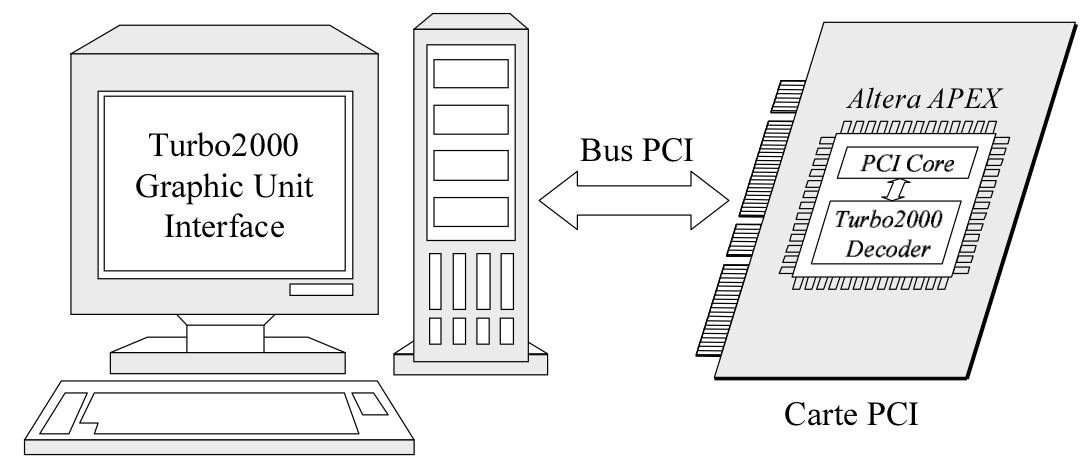
\includegraphics[width=0.9\textwidth]{images/figura4_3}
\caption{Plataforma Turbo2000.}
\label{fig:4.3}
\end{figure}

\section{Tablas}
\noindent
Esta secci'on presenta algunos ejemplos de formatos de tablas extra'idas de la referencia \cite{Demo:phdTesis} que se pueden usar en el documento de tesis.
\begin{table}[H]
	\begin{center}
		\begin{tabular}{ | c | c | c | }
			\hline
			& & \\[-18pt]
			\emph{q} bits	&	\emph{L}\subscript{max}	&	\begin{math}\Delta\end{math}\subscript{max} \\[3pt]
			\hline \hline
			& & \\[-18pt]
			2 & 11 & 8 \\[8pt]
			3 & 33 & 24 \\[8pt]
			4 & 77 & 82 \\[8pt]
			5 & 165 & 123 \\[8pt]
			6 & 341 & 395 \\[5pt]
			\hline
		\end{tabular}
	\end{center}
	\caption{Din'amica de m'etricas para diferentes valores de q con $R =1/2, E_b/N_0 = 2 dB$ y modulaci'on QPSK.}
\end{table}

\begin{table}[H]
	\begin{center}
	\begin{threeparttable}
	\begin{tabular}{ | c || c | c | }
		\hline
		& & \\[-8pt]
		Unit'e	&	\# Add./Soustr.	&	\# min(.)	\\[3pt]
		\hline \hline
		& & \\[-18pt]CMB			&	22					&	0					\\& & \\[-18pt]\hline
		& & \\[-18pt]Proc. ACS		&	$2^m \cdot N_a = 64$	&	$N_s \cdot (2^m-1)=48$	\\& & \\[-18pt]\hline
		& & \\[-18pt]CP			&	$2^m \cdot N_a = 64$	&	$2^m \cdot (N_s-1)=60$	\\& & \\[-18pt]\hline
		& & \\[-18pt]CIE\tnote{a}	&	$2^{m+1} = 8$		&	$2^m-1=3$			\\& & \\[-18pt]\hline
		& & \\[-18pt]CCD\tnote{b}	&	1					&	2					\\& & \\[-18pt]\hline
		& & \\[-18pt]CCA\tnote{b}	&	1					&	2					\\
		\hline
	\end{tabular}
	\setstretch{1.0}
	\begin{tablenotes}
		\item[\tiny a]{\tiny No se consideran los sub-bloques de actualizaci'on de los datos extr'insecos.}
		\item[\tiny b]{\tiny El comparador de salida es considerado como un sumador.}
	\end{tablenotes}
	\setstretch{1.5}
	\end{threeparttable}
	\end{center}
	\caption{Complejidad de c'alculo de las unidades del decodificador Turbo2000.}
\end{table}

\begin{table}[H]
	\begin{center}
	\begin{threeparttable}
	\begin{tabular}{ | l || l | l | l |}
		\hline
		& & & \\[-18pt]
		\textbf{Tratamiento}		&	\textbf{Unidades activas}		&	\textbf{\# Add./Soustr.}	&	\textbf{\# min(.)}	\\[3pt]
		\hline \hline
		& & &\\[-18pt]RETOUR 2	&	CMB, Proc. ACS \emph{Retour}&	$22+2^m \cdot N_s$			& $N_s \cdot (2^m-1)$\\& & &\\[-18pt]
		& & &\\[-18pt]			&						&	86						& 48\\& & &\\[-18pt]\hline
		& & &\\[-18pt]ALLER 2		&	CMB, Proc. ACS \emph{Aller},&	$22+2^{m+1} \cdot (N_s+1)$	& $N_s \cdot (2^m-1)-1$\\& & &\\[-18pt]
		& & &\\[-18pt]			&	CP, CIE				&	158						& 111\\& & &\\[-18pt]\hline
		& & &\\[-18pt]RETOUR 1	&	CMB, Proc. ACS \emph{Retour}&	$22+2^m \cdot N_s$			& $N_s \cdot (2^m-1)$\\& & &\\[-18pt]
		& & &\\[-18pt]			&						&	86						& 48\\& & &\\[-18pt]\hline
		& & &\\[-18pt]ALLER 1		&	CMB, Proc. ACS \emph{Aller},&	$24+2^{m+1} \cdot (N_s+1)$	& $N_s \cdot (2^m-1)+3$\\& & &\\[-18pt]
		& & &\\[-18pt]			&	CP, CIE, CDD, CCA			&	160						& 115\\[3pt]
		\hline
	\end{tabular}
	\end{threeparttable}
	\end{center}
	\caption{Complejidad de c'alculo seg'un el tratamiento del decodificador Turbo2000.}
\end{table}

\section{M'argenes}
\noindent
\begin{enumerate}
	\item El margen izquierdo (del lado del encuadernado) ser'a de tres cent'imetros, incluyendo tablas e ilustraciones. El margen derecho ser'a de dos cent'imetros.
	\item Los m'argenes superior e inferior ser'an de dos cent'imetros. Esto no incluye los encabezados o pies de p'agina.
	\item Las p'aginas horizontales deber'an tener en la parte superior de la hoja un margen de tres cent'imetros; para que, al ubicarlas de manera vertical en el manuscrito, este margen coincida con el requerido para el encuadernado.
\end{enumerate}

\section{Espacios}
\noindent
\begin{enumerate}
	\item El texto del trabajo se har'a a doble espacio como viene en este manual.
	\item Se permite usar espacio sencillo en el 'indice de contenido, de ilustraciones, de tablas y en los ap'endices.
	\item El espacio sencillo es obligatorio para citas textuales en p'arrafos de otros autores, pies de figura, pies de tabla y pies de p'agina. Ejemplo de una cita textual \cite{Demo:phdTesis}:\\
	
	\setstretch{1.0}
	\small
	``Un turbo-c'odigo m-binario est'a compuesto de dos c'odigos CRSC m-binarios id'enticos concatenados en paralelo a trav'es de un permutador. La t'ecnica de terminaci'on circular es utilizada en estos c'odigos bidimensionales para codificar bloques sin hacer uso de bits de terminaci'on. La tasa de codificaci'on global R para un turbo-c'odigo es igual a m/(m + 2).''
\end{enumerate}
\setstretch{1.5}

\section{P'aginas}
\noindent
\begin{enumerate}
	\item Se numeran todas las p'aginas a partir de las p'aginas de Dedicatoria, Agradecimientos, Resumen, Contenido, Lista de Tablas y Figuras, Bibliograf'ia, Ap'endices y Vitae.
	\item No se numeran las p'aginas de la Portada y de Firmas.
	\item Coloca los n'umeros de p'aginas en el centro del margen inferior al inicio de un cap'itulo, y en el margen superior derecho para las dem'as. Las p'aginas en las que aparecen cuadros y gr'aficas tambi'en deben numerarse y su disposici'on (vertical u horizontal) no debe alterar la posici'on del n'umero de p'agina.
	\item Las p'aginas que incluyen la Dedicatoria, Agradecimientos, Resumen, Contenido, Lista de Tablas y Figuras utilizan la numeraci'on romana, es decir, I, II, III, IV, etc.
	\item Las p'aginas a partir del cap'itulo 1 utilizan la numeraci'on ar'abiga, es decir, 1, 2, 3, etc. Esto considera tambi'en a la Bibliograf'ia, los Ap'endices y el Vitae.
	\item No uses la palabra ``p'agina'' antes de la numeraci'on de las p'aginas.
	\item Usa el mismo tipo de letra para todos los n'umeros de p'agina.
\end{enumerate}

\section{Manuscrito final del documento de tesis}
\noindent
El manuscrito final de tesis deber'a respetar el siguiente orden:
\begin{enumerate}
	\item Portada del empastado (obligatoria): No se coloca el n'umero de p'agina y no se cuenta. Ver primera p'agina del manual.
	\item P'agina de Firmas (obligatoria): No se coloca el n'umero de p'agina y no se cuenta. Ver segunda p'agina del manual.
	\item Dedicatoria (opcional): Se coloca p'agina con n'umero romano en min'uscula.
	\item Ep'igrafe (opcional): Se coloca p'agina con n'umero romano en min'uscula.
	\item P'agina de reconocimientos o agradecimientos (opcional): Se coloca p'agina con n'umero romano en min'uscula.
	\item Resumen (obligatorio): Se coloca p'agina con n'umero romano en min'uscula.
	\item 'Indice de contenido (obligatorio): Se coloca p'agina con n'umero romano en min'uscula.
	\item Lista de tablas (puede ser requerido): Se coloca p'agina con n'umero romano en min'uscula.
	\item Lista de ilustraciones o gr'aficas (puede ser requerido): Se coloca p'agina con n'umero romano en min'uscula.
	\item Lista de abreviaturas (opcional): Se coloca p'agina con n'umero romano en min'uscula.
	\item Glosario (opcional): Se coloca p'agina con n'umero romano en min'uscula.
	\item Introducci'on (obligatoria). La introducci'on ser'a considerada como el primer cap'itulo del cuerpo del manuscrito. A partir de aqu'i inicia la paginaci'on ar'abiga.
	\item Cuerpo del manuscrito (obligatorio): Continu'a la paginaci'on ar'abiga.
	\newpage
	\item Referencias bibliogr'aficas (obligatorio): Continu'a la paginaci'on ar'abiga. Utilizar el formato del IEEE como viene en la siguiente p'agina.
	\item Ap'endices (opcional): Continu'a la paginaci'on ar'abiga.
	\item Vitae (obligatorio): Continu'a la paginaci'on ar'abiga.
\end{enumerate}

\clearpage

	%Empieza configuracion de capitulo
\setstretch{1.0}
\titleformat{\chapter}[block]{\Large\bfseries}{CHAPTER \Huge\thechapter\vspace{25 pt}}{0 pt}{\\\fontsize{26}{36}\selectfont}
\titlespacing{\chapter}{0 pt}{30 pt}{50 pt}[0 pt]
\titleformat{\section}{\Large\bfseries}{\thesection}{0 pt}{\hspace{30 pt}}
\titleformat{\subsection}{\large\bfseries}{\thesubsection}{0 pt}{\hspace{30 pt}}
\pagestyle{fancy}
\fancyhead[LO,LE]{\footnotesize\emph{\leftmark}}
\fancyhead[RO,RE]{\thepage}
\fancyfoot[CO,CE]{}
%Termina configuracion de capitulo

\chapter{Experiments}
\setstretch{1.5} %Regresa el interlineado a 1.5

\normalsize
\noindent

\section{Find the correct OS}
\noindent

    The first approach was to find the correct Operating system for the test,
    however this wasn't easy in the beginning we started to create a few
    experiments. In the end we came up with a full support of MPi for embedded
    platforms support that the community thanks to us a lot.

    \subsection {Embedded Distributed Systems: A Case of Study with Clear Linux
    Project for Intel Architecture}
    \noindent



The main objective of this work will be to prove that a distributed embedded
system (Intel® Atom-TM Processor E3825) running real HPC workloads 
(MPI benchmarks) can be improved by the use of a customized operating system 



The need of more complex and smart applications (they must adapt their
performance as well as power) has risen the bar to create distributed systems
based on parallel embedded platforms. 

By definition: A distributed system consists of a collection of autonomous
computers, connected through a network and distribution middle-ware, which
enables computers to coordinate their activities and to share the resources of
the system, so that users perceive the system as a single, integrated computing
facility.

Advantages: 

\begin{enumerate} 
    
    \item \textbf{Partitioning Workload}: 
    By partitioning the workload onto multiple processors, 
    each processor is now responsible for only a fraction of the workload. 
    The processors can now afford to slow down by dynamic voltage scaling 
    (DVS) to run at more power-efficient states, and the degraded performance 
    on each processor can still contribute to an increased system-wide 
    performance by the increased parallelism.  

    \item \textbf{Heterogeneous HW}: 
    Another advantage with a distributed scheme is that heterogeneous hardware 
    such as DSP and other accelerators can further improve power efficiency 
    of various stages of the computation through specialization.

\end{enumerate}
 

Disadvantages: 

\begin{enumerate}
    \item \textbf{Network}: Despite the fact the distributed systems may have
    many attractive properties, they pay a higher price for message-passing 
    communications. Each node now must handle not only communication with 
    the external world, but also extra communication on the internal network. 
    As a result, even if the actual data payload is not large on an absolute 
    scale, the communication appears very expensive and does not scale to a few
    more nodes

    \item \textbf{Lack of optimized OS}: A typical embedded system often does
    not contain an operating system. Crafting distributed programs on such a
    bare-bone platform is extremely difficult and error-prone. Although many
    higher-level abstractions such as Message Passing Interfaces (MPI) have been
    proposed to facilitate distributed programming, these abstraction layers require
    extensive system resources with comprehensive operating systems support, which
    may not be available to an embedded platform 
    
\end{enumerate}
 
However in recent years we have seen an emergence of a new class of full-fledged
embedded systems (they are fully loaded with sufficient system resources as well
as networking and other peripheral devices, and a complete version of the
operating system with network support) In addition, they are typically designed
with power-management technology in order to extend the battery life

With these gaps closed there might be a chance to merge the parallel and
distributed paradigms on the embedded world.  A merging point of technologies
from different domains often inspires technology innovations in new domains.

\section{Development}

According to these in consideration there are multiple scenarios to test the
capability of an embedded distributed system: 


\begin{itemize} 
    
    \item Compare an Embedded system with generic SW (Linux base OS
    (Fedora/Ubuntu/Debian) and generic MPI protocol (MPICH)) against a
    regular development system (with the same OS and MPI tools)

    \item Compare an Embedded system with a distributed operating system
    against the same embedded system with custom SW (Linux from scratch system)


    \item Compare an Embedded system with a distributed operating system
    against the same embedded system with custom SW (Linux from scratch system and
    MPI for embedded (LMPI)) in order to check the gap in the multiple systems

\end{itemize}

For this report we will execute the experiment of the second scenario, due to the
fact that we have already done the study of the first scenario. In that case we
realize that despite the fact that the minnow Max ran 8 times slower than the
regular development system (NUC Haswell system) the Minnow Max was more stable
and with less drops in performance. 

The operating system we will use is the Fedora 19 system, the description of the
system is listed on the fedora project site home page (http://fedoraproject.org)

The benchmark we will use to measure the performance is MPIbench. This is a
program to measure the performance of some critical MPI functions. By critical
it means that the behavior of these functions can dominate the run time of a
distributed application. MP-Bench has now been integrated into LLCbench (Low
Level Characterization Benchmarks) 

The MPIfunctions that it stress are: 


\begin{itemize}

\item MPI\_Send/MPI\_Recv Bandwidth (Kb/second vs. bytes) 
\item MPI\_Send/MPI\_Recv Application latency or Gap time (us vs. bytes)
\item MPI\_Send/MPI\_Recv Roundtrip or 2 * Latency (trns/second vs. bytes) 
\item MPI\_Send/MPI\_Recv() BidirectionalBandwidth (Kb/second vs. bytes) 
\item MPI\_Bcast broadcast (Kb/second vs. bytes) 
\item MPI\_Reduce reduction (sum) (Kb/second vs. bytes) 
\item MPI\_AllReduce reduction (sum) (Kb/second vs. bytes) 
\item MPI\_Alltoall Each process sends to every other process (Kb/sec vs. bytes) 

\end{itemize}


    \subsection {Embedded Distributed Systems: A Case of Study with Yocto project}
    \noindent

\section{Find the correct MPI protocol configuration}
\noindent

\section{Embedded Distributed System: A case of study in smart greenhouses}
\noindent

\section{Embedded Distributed System: PnP measurement with comercial OS}
\noindent

\clearpage

	%Empieza configuracion de capitulo
\setstretch{1.0}
\titleformat{\chapter}[block]{\Large\bfseries}{CAP'ITULO \Huge\thechapter\vspace{25 pt}}{0 pt}{\\\fontsize{26}{36}\selectfont}
\titlespacing{\chapter}{0 pt}{30 pt}{50 pt}[0 pt]
\titleformat{\section}{\Large\bfseries}{\thesection}{0 pt}{\hspace{30 pt}}
\titleformat{\subsection}{\large\bfseries}{\thesubsection}{0 pt}{\hspace{30 pt}}
\pagestyle{fancy}
\fancyhead[LO,LE]{\footnotesize\emph{\leftmark}}
\fancyhead[RO,RE]{\thepage}
\fancyfoot[CO,CE]{}
%Termina configuracion de capitulo

\chapter{Conclusions}
\setstretch{1.5} %Regresa el interlineado a 1.5

\normalsize
\noindent

\section{Conclusions}
\noindent

In this thesis work it was proposed the hypothesis that a cluster of ultra-low
power IoT platforms can be as computing powerful and energy efficient as a
traditional computing system.

In chapter one we present a simulation to illustrate such hypothesis. It is described in
Figure~\ref{fig:1.2}.  At the beginning , the increment in the number of nodes
in the studied network produces an increment on performance; however, it is
expected to reach a maximum point at which power efficiency becomes stable and
it will remain in such state up to a certain point at which it will start to
decrease. 

As we can see in the previous graphs this behavior was achieved as expected. At
the number of platforms increases it is expected the performance benefit
increase, because the amount of work to be done is distributed among different
platforms, but as more are added due to the power they consume the performance
gain starts to minimize. When the ideal number of platforms is exceeded, the
power efficiency decrease rapidly.

In all the experiment we realize, the ideal number of platforms is always
between three and four. This gave us the confidence to say that as a conclusion
that the energy efficiency (using MPI Benchmarks as a reference workload) of an
IoT distributed system is similar to a traditional computing system \cite{NUC}
with three or four nodes.

\section{Future Work}
\noindent

\clearpage

	%Empieza configuracion de capitulo
\setstretch{1.0}
\titleformat{\chapter}[block]{\Large\bfseries}{CAP'ITULO \Huge\thechapter\vspace{25 pt}}{0 pt}{\\\fontsize{26}{36}\selectfont}
\titlespacing{\chapter}{0 pt}{30 pt}{50 pt}[0 pt]
\titleformat{\section}{\Large\bfseries}{\thesection}{0 pt}{\hspace{30 pt}}
\titleformat{\subsection}{\large\bfseries}{\thesubsection}{0 pt}{\hspace{30 pt}}
\pagestyle{fancy}
\fancyhead[LO,LE]{\footnotesize\emph{\leftmark}}
\fancyhead[RO,RE]{\thepage}
\fancyfoot[CO,CE]{}
%Termina configuracion de capitulo

\chapter{Results}
\setstretch{1.5} %Regresa el interlineado a 1.5

\normalsize
\noindent

\section{Find the correct OS}
\noindent

    \subsection {Embedded Distributed Systems: A Case of Study with Clear Linux
    Project for Intel® Architecture}
    \noindent

    \subsection {Embedded Distributed Systems: A Case of Study with Yocto project}
    \noindent

\section{Find the correct MPI protocol configuration}
\noindent

\section{Embedded Distributed System: A case of study in smart greenhouses}
\noindent

\section{Embedded Distributed System: PnP measurement with comercial OS}
\noindent

\clearpage

	%Empieza configuracion de capitulo
\setstretch{1.0}
\titleformat{\chapter}[block]{\Large\bfseries}{CAP'ITULO \Huge\thechapter\vspace{25 pt}}{0 pt}{\\\fontsize{26}{36}\selectfont}
\titlespacing{\chapter}{0 pt}{30 pt}{50 pt}[0 pt]
\titleformat{\section}{\Large\bfseries}{\thesection}{0 pt}{\hspace{30 pt}}
\titleformat{\subsection}{\large\bfseries}{\thesubsection}{0 pt}{\hspace{30 pt}}
\pagestyle{fancy}
\fancyhead[LO,LE]{\footnotesize\emph{\leftmark}}
\fancyhead[RO,RE]{\thepage}
\fancyfoot[CO,CE]{}
%Termina configuracion de capitulo

\chapter{Conclusions}
\setstretch{1.5} %Regresa el interlineado a 1.5

\normalsize
\noindent

\section{Conclusions}
\noindent

    \subsection {Embedded Distributed Systems: A Case of Study with Clear Linux
    Project for Intel® Architecture}
    \noindent

    \subsection {Embedded Distributed Systems: A Case of Study with Yocto project}
    \noindent

    \subsection{Find the correct MPI protocol configuration}
    \noindent

    \subsection{Embedded Distributed System: A case of study in smart greenhouses}
    \noindent

    \subsection{Embedded Distributed System: PnP measurement with comercial OS}
    \noindent


\section{Future Work}
\noindent

\clearpage


	%Empieza configuracion
\setstretch{1.0}
\titleformat{\chapter}{\Huge\bfseries}{\thechapter}{0 pt}{\rule{340 pt}{3 pt}\\}
\titlespacing{\chapter}{100 pt}{-25 pt}{40 pt}[10 pt]	
\pagestyle{fancy}
\fancyhead[RO,RE]{\thepage}
\fancyfoot[CO,CE]{}
%Termina configuracion

\setstretch{1.5}
\nocite{Benkhelifa}

\nocite{Wun}

\bibliographystyle{includes/IEEEtranBST/IEEEtran}
\bibliography{includes/tesis}
\addcontentsline{toc}{chapter}{Bibliograf'ia}


	\appendix
	%Empieza configuracion de capitulo
\setstretch{1.0}
\titleformat{\chapter}[block]{\Large\bfseries}{AP'ENDICE \Huge\thechapter\vspace{25 pt}}{0 pt}{\\\fontsize{26}{36}\selectfont}
\titlespacing{\chapter}{0 pt}{30 pt}{50 pt}[0 pt]
\titleformat{\section}{\Large\bfseries}{\thesection}{0 pt}{\hspace{30 pt}}
\titleformat{\subsection}{\large\bfseries}{\thesubsection}{0 pt}{\hspace{30 pt}}
\pagestyle{fancy}
\fancyhead[LO,LE]{\footnotesize\emph{\leftmark}}
\fancyhead[RO,RE]{\thepage}
\fancyfoot[CO,CE]{}
%Termina configuracion de capitulo

\chapter{Procedimientos de Defensa de la Propuesta} %Cambia al nombre de tu capitulo
\setstretch{1.5} %Regresa el interlineado a 1.5

\normalsize
Una vez que se ha redactado la propuesta, debe entregarla al director para que la firme. Se recomienda hacer dos copias del documento, una para usted y otra para la direcci'on de maestr'ia.

	%Empieza configuracion de capitulo
\setstretch{1.0}
\titleformat{\chapter}[block]{\Large\bfseries}{AP'ENDICE \Huge\thechapter\vspace{25 pt}}{0 pt}{\\\fontsize{26}{36}\selectfont}
\titlespacing{\chapter}{0 pt}{30 pt}{50 pt}[0 pt]
\titleformat{\section}{\Large\bfseries}{\thesection}{0 pt}{\hspace{30 pt}}
\titleformat{\subsection}{\large\bfseries}{\thesubsection}{0 pt}{\hspace{30 pt}}
\pagestyle{fancy}
\fancyhead[LO,LE]{\footnotesize\emph{\leftmark}}
\fancyhead[RO,RE]{\thepage}
\fancyfoot[CO,CE]{}
%Termina configuracion de capitulo

\chapter{'Ultimos Detalles} %Cambia al nombre de tu capitulo
\setstretch{1.5} %Regresa el interlineado a 1.5

\normalsize
Aqu'i vienen los detalles que no se mencionaron en el cuerpo del contenido para alg'un tema espec'ifico.

	%Empieza configuracion
\setstretch{1.0}
\titleformat{\chapter}{\Huge\bfseries}{\thechapter}{0 pt}{\rule{340 pt}{3 pt}\\}
\titlespacing{\chapter}{100 pt}{-25 pt}{40 pt}[10 pt]	
\pagestyle{fancy}
\fancyhead[RO,RE]{\thepage}
\fancyfoot[CO,CE]{}
%Termina configuracion

\chapter*{Vitae}
\addcontentsline{toc}{chapter}{Vitae}
\setstretch{1.5} %Regresa el interlineado a 1.5

\normalsize
\noindent

\end{document}

% Template de LaTex para tesis del ITESM Campus Guadalajara
% Basado en el template de Word de Ra\'ul Crespo Saucedo
% Basado en el sistema de guiones de Universidad Computense de Madrid
% Adaptaci\'on realizada por Arturo Jafet Rodr\'iguez Mu\'noz
% Revision por Marco Antonio Rangel Bocardo
% Maestr\'ia en Ciencias Computacionales - ITESM Campus Guadalajara
% Guadalajara, Jalisco Septiembre del 2011
% Recomiendo esta gu'ia de LaTex: http://en.wikibooks.org/wiki/LaTeX/

\documentclass[12pt,letterpaper]{report}
\usepackage[english,spanish,activeacute]{babel}
\usepackage[T1]{fontenc}
\usepackage{dirtytalk}
\usepackage{graphicx}
\usepackage[letterpaper]{geometry}
\usepackage{titlesec}
\usepackage{fancyhdr}
\usepackage{fix-cm}
\usepackage{setspace} 
\usepackage{amsmath}
\usepackage{fmtcount}
\usepackage{threeparttable}
\usepackage{float}
\usepackage{mathtools}

\usepackage{graphicx}
\usepackage[table]{xcolor}
\usepackage{listings}

\usepackage[font=small,format=plain,labelfont=bf,it]{caption}
\geometry{top=2.5cm, bottom=2.5cm, left=3.0cm, right=2.5cm}
\renewcommand{\rmdefault}{cmr} % Roman
\renewcommand{\encodingdefault}{T1}
\newcommand{\subscript}[1]{\ensuremath{_{\textrm{#1}}}}
\setstretch{1.5}

\usepackage{hyperref}


%\headheight = 49pt
%\footskip = 10pt


%----------------------------------------------------------------
%
% Fichero con algunas divisiones de palabras que LaTeX no
% hace correctamente si no se le da alguna ayuda.
%
% Universidad Computense de Madrid
% http://gaia.fdi.ucm.es/projects/texis
%----------------------------------------------------------------

\hyphenation{
% a
abs-trac-to
abs-trac-tos
abs-trac-ta
abs-trac-tas
ac-tua-do-res
a-gra-de-ci-mien-tos
ana-li-za-dor
an-te-rio-res
an-te-rior-men-te
apa-rien-cia
a-pro-pia-do
a-pro-pia-dos
a-pro-pia-da
a-pro-pia-das
a-pro-ve-cha-mien-to
a-que-llo
a-que-llos
a-que-lla
a-que-llas
a-sig-na-tu-ra
a-sig-na-tu-ras
a-so-cia-da
a-so-cia-das
a-so-cia-do
a-so-cia-dos
au-to-ma-ti-za-do
% b
batch
bi-blio-gra-f\'ia
bi-blio-gr\'a-fi-cas
bien
bo-rra-dor
boo-l-ean-expr
% c
ca-be-ce-ra
call-me-thod-ins-truc-tion
cas-te-lla-no
cir-cuns-tan-cia
cir-cuns-tan-cias
co-he-ren-te
co-he-ren-tes
co-he-ren-cia
co-li-bri
co-men-ta-rio
co-mer-cia-les
co-no-ci-mien-to
cons-cien-te
con-si-de-ra-ba
con-si-de-ra-mos
con-si-de-rar-se
cons-tan-te
cons-trucci\'on
cons-tru-ye
cons-tru-ir-se
con-tro-le
co-rrec-ta-men-te
co-rres-pon-den
co-rres-pon-dien-te
co-rres-pon-dien-tes
co-ti-dia-na
co-ti-dia-no
crean
cris-ta-li-zan
cu-rri-cu-la
cu-rri-cu-lum
cu-rri-cu-lar
cu-rri-cu-la-res
% d
de-di-ca-do
de-di-ca-dos
de-di-ca-da
de-di-ca-das
de-rro-te-ro
de-rro-te-ros
de-sa-rro-llo
de-sa-rro-llos
de-sa-rro-lla-do
de-sa-rro-lla-dos
de-sa-rro-lla-da
de-sa-rro-lla-das
de-sa-rro-lla-dor
de-sa-rro-llar
des-cri-bi-re-mos
des-crip-ci\'on
des-crip-cio-nes
des-cri-to
des-pu\'es
de-ta-lla-do
de-ta-lla-dos
de-ta-lla-da
de-ta-lla-das
di-a-gra-ma
di-a-gra-mas
di-se-�os
dis-po-ner
dis-po-ni-bi-li-dad
do-cu-men-ta-da
do-cu-men-to
do-cu-men-tos
% e
edi-ta-do
e-du-ca-ti-vo
e-du-ca-ti-vos
e-du-ca-ti-va
e-du-ca-ti-vas
e-la-bo-ra-do
e-la-bo-ra-dos
e-la-bo-ra-da
e-la-bo-ra-das
es-co-llo
es-co-llos
es-tu-dia-do
es-tu-dia-dos
es-tu-dia-da
es-tu-dia-das
es-tu-dian-te
e-va-lua-cio-nes
e-va-lua-do-res
exis-ten-tes
exhaus-ti-va
ex-pe-rien-cia
ex-pe-rien-cias
% f
for-ma-li-za-do
% g
ge-ne-ra-ci\'on
ge-ne-ra-dor
ge-ne-ra-do-res
ge-ne-ran
% h
he-rra-mien-ta
he-rra-mien-tas
% i
i-dio-ma
i-dio-mas
im-pres-cin-di-ble
im-pres-cin-di-bles
in-de-xa-do
in-de-xa-dos
in-de-xa-da
in-de-xa-das
in-di-vi-dual
in-fe-ren-cia
in-fe-ren-cias
in-for-ma-ti-ca
in-gre-dien-te
in-gre-dien-tes
in-me-dia-ta-men-te
ins-ta-la-do
ins-tan-cias
% j
% k
% l
len-gua-je
li-be-ra-to-rio
li-be-ra-to-rios
li-be-ra-to-ria
li-be-ra-to-rias
li-mi-ta-do
li-te-ra-rio
li-te-ra-rios
li-te-ra-ria
li-te-ra-rias
lo-tes
% m
ma-ne-ra
ma-nual
mas-que-ra-de
ma-yor
me-mo-ria
mi-nis-te-rio
mi-nis-te-rios
mo-de-lo
mo-de-los
mo-de-la-do
mo-du-la-ri-dad
mo-vi-mien-to
% n
na-tu-ral
ni-vel
nues-tro
% o
obs-tan-te
o-rien-ta-do
o-rien-ta-dos
o-rien-ta-da
o-rien-ta-das
% p
pa-ra-le-lo
pa-ra-le-la
par-ti-cu-lar
par-ti-cu-lar-men-te
pe-da-g\'o-gi-ca
pe-da-g\'o-gi-cas
pe-da-g\'o-gi-co
pe-da-g\'o-gi-cos
pe-rio-di-ci-dad
per-so-na-je
plan-te-a-mien-to
plan-te-a-mien-tos
po-si-ci\'on
pre-fe-ren-cia
pre-fe-ren-cias
pres-cin-di-ble
pres-cin-di-bles
pri-me-ra
pro-ble-ma
pro-ble-mas
pr\'o-xi-mo
pu-bli-ca-cio-nes
pu-bli-ca-do
% q
% r
r\'a-pi-da
r\'a-pi-do
ra-zo-na-mien-to
ra-zo-na-mien-tos
re-a-li-zan-do
re-fe-ren-cia
re-fe-ren-cias
re-fe-ren-cia-da
re-fe-ren-cian
re-le-van-tes
re-pre-sen-ta-do
re-pre-sen-ta-dos
re-pre-sen-ta-da
re-pre-sen-ta-das
re-pre-sen-tar-lo
re-qui-si-to
re-qui-si-tos
res-pon-der
res-pon-sa-ble
% s
se-pa-ra-do
si-guien-do
si-guien-te
si-guien-tes
si-guie-ron
si-mi-lar
si-mi-la-res
si-tua-ci\'on
% t
tem-pe-ra-ments
te-ner
trans-fe-ren-cia
trans-fe-ren-cias
% u
u-sua-rio
Unreal-Ed
% v
va-lor
va-lo-res
va-rian-te
ver-da-de-ro
ver-da-de-ros
ver-da-de-ra
ver-da-de-ras
ver-da-de-ra-men-te
ve-ri-fi-ca
% w
% x
% y
% z
}
% Variable local para emacs, para que encuentre el fichero
% maestro de compilaci\'on
%%%
%%% Local Variables:
%%% mode: latex
%%% TeX-master: "./Tesis.tex"
%%% End:


\begin{document}
	\renewcommand{\tablename}{Tabla}

	\pagestyle{empty}
\begin{center}
\begin{center}

\includegraphics[scale=0.5]{images/escudo-itesm_small.png}
\end{center}
\vspace{17 pt}
\renewcommand{\baselinestretch}{1.0}
\Huge
%\textbf{I\hspace{1pt}n\hspace{1pt}s\hspace{1pt}t\hspace{1pt}i\hspace{1pt}t\hspace{1pt}u\hspace{1pt}t\hspace{1pt}o\hspace{1pt} \hspace{1pt}T\hspace{1pt}e\hspace{1pt}c\hspace{1pt}n\hspace{1pt}o\hspace{1pt}l\hspace{1pt}'o\hspace{1pt}g\hspace{1pt}i\hspace{1pt}c\hspace{1pt}o\hspace{1pt} \hspace{1pt}y \hspace{1pt}d\hspace{1pt}e\hspace{1pt} \hspace{1pt}E\hspace{1pt}s\hspace{1pt}t\hspace{1pt}u\hspace{1pt}d\hspace{1pt}i\hspace{1pt}o\hspace{1pt}s\\ S\hspace{1pt}u\hspace{1pt}p\hspace{1pt}e\hspace{1pt}r\hspace{1pt}i\hspace{1pt}o\hspace{1pt}r\hspace{1pt}e\hspace{1pt}s\hspace{1pt} \hspace{1pt}d\hspace{1pt}e\hspace{1pt} \hspace{1pt}M\hspace{1pt}o\hspace{1pt}n\hspace{1pt}t\hspace{1pt}e\hspace{1pt}r\hspace{1pt}r\hspace{1pt}e\hspace{1pt}y}\\
\textbf{Instituto Tecnol'ogico y de Estudios\\Superiores de Monterrey}\\
\LARGE
\textbf{Campus Guadalajara}\\
\vspace{11 pt}

\Large
\textbf{Escuela de Graduados en Ingenier'ia y\\ Arquitectura (EGIA)}\\
\vspace{20 pt}

\textbf{Maestr'ia en Ciencias Computacionales}\\
\vspace{42 pt}

\Huge
\textbf{Methodology for design of self sustainable IoT network}\\
\vspace{65 pt}

\Large
\begin{flushleft}
\hspace{5pt}\textbf{AUTOR: Victor Manuel Rodriguez Bahena}\\
\vspace{5pt}
\hspace{5pt}\textbf{ASESORES:PhD Marcos de Alba} \\
\end{flushleft}

\large
\vspace{20pt}
\textbf{Guadalajara (Jal), 10 de Mayo de 2015}
\end{center}
\clearpage

\renewcommand{\baselinestretch}{1.5}


	\pagenumbering{roman}
	%Empieza configuracion
\setstretch{1.0}
\titleformat{\chapter}{\Huge\bfseries}{\thechapter}{0 pt}{\rule{340 pt}{3 pt}\\}
\titlespacing{\chapter}{100 pt}{-25 pt}{40 pt}[10 pt]	
\pagestyle{fancy}
\fancyhead[RO,RE]{\thepage}
\fancyfoot[CO,CE]{}
%Termina configuracion

\chapter*{Acknowledgments}
\addcontentsline{toc}{chapter}{Acknowledgments}
\setstretch{1.5} %Regresa el interlineado a 1.5

\vspace{140 pt}

\normalsize
\begin{flushright}
\textit{First and foremost, I have to thank my parents for their love and support
throughout my life. My brother and loved ones deserve my wholehearted thanks as
well. Thank you for your understanding, patience and encouragement in many
difficult moments.}

\textit{I would like to express my sincere gratitude to my advisor PhD.
Marcos Ruben de Alba Rosano for the continuous support of my master degree 
study and related research, for  his patience, motivation,
and immense knowledge.}

\textit{I would like to sincerely thank Intel company as well as the Instituto
Tecn\'ologico y de Estudios Superiores de Monterrey for his support with the
scholarship and support to finish this achievement in my life.}

\end{flushright}
\clearpage

	%Empieza configuracion
\setstretch{1.0}
\titleformat{\chapter}{\Huge\bfseries}{\thechapter}{0 pt}{\rule{340 pt}{3 pt}\\}
\titlespacing{\chapter}{100 pt}{-25 pt}{40 pt}[10 pt]	
\pagestyle{fancy}
\fancyhead[RO,RE]{\thepage}
\fancyfoot[CO,CE]{}
%Termina configuracion

\chapter*{Acknowledgments}
\addcontentsline{toc}{chapter}{Acknowledgments}
\setstretch{1.5} %Regresa el interlineado a 1.5

\normalsize
\noindent
\clearpage

	%Empieza configuracion
\setstretch{1.0}
\titleformat{\chapter}{\Huge\bfseries}{\thechapter}{0 pt}{\rule{340 pt}{3 pt}\\}
\titlespacing{\chapter}{100 pt}{-25 pt}{40 pt}[10 pt]	
\pagestyle{fancy}
\fancyhead[RO,RE]{\thepage}
\fancyfoot[CO,CE]{}
%Termina configuracion

\chapter*{Resumen}
\addcontentsline{toc}{chapter}{Resumen}
\setstretch{1.5} %Regresa el interlineado a 1.5


\normalsize
\noindent El resumen es una s'intesis de la tesis. Generalmente incluir'a la definici'on del problema, el procedimiento o m'etodos, los resultados y las conclusiones. Esta secci'on deber'a tener un m'aximo de trescientas cincuenta palabras incluyendo preposiciones. Las palabras en el t'itulo no se cuentan como parte del resumen. El resumen debe escribirse con claridad, ya que 'esta es la referencia que se hace p'ublica inmediatamente en los servicios electr'onicos de b'usqueda de informaci'on. Deber'a escribirse a doble espacio. No se recomienda usar diagramas ni f'ormulas en esta secci'on.

En este documento se presenta la estructura de la propuesta de tesis que los alumnos del curso Seminario de Innovaci'on y Creatividad deben presentar para acreditar la materia. Se describen los elementos de la propuesta y el formato que dichos elementos deben llevar. En la portada debe ir el t'itulo tentativo de la tesis, el nombre del autor, la instituci'on de educaci'on superior en la que se realiza el trabajo de tesis, el mes y a'no en que se entreg'o la propuesta. Despu'es de la portada va una p'agina de aprobaci'on que debe ser firmada por el director de la tesis y los sinodales una vez el proyecto haya sido aprobado. En el caso que el documento sea una propuesta de tesis, se debe llenar el formato de Registro de Tesis que se debe entregar a Servicios Escolares antes de que termine el seminario. Este Registro es una condici'on necesaria para que el alumno pueda inscribirse a la materia que sigue: Tesis I.

Posteriormente, puede seguir una dedicatoria que es de car'acter opcional y una secci'on de reconocimientos en la que deben mencionarse aquellas instituciones o personas, si las hay, que est'en proporcionando ayuda o apoyo financiero al proyecto. Por 'ultimo sigue el resumen de la tesis, cuya extensi'on debe ser de una p'agina a dos p'aginas m'aximo.

El contenido muestra las diferentes secciones y cap'itulos de la tesis. Las p'aginas se indican con numeraci'on ar'abiga comenzando desde el cap'itulo 1. Las p'aginas de todas las secciones anteriores al cap'itulo 1 se identifican con numeraci'on romana. Si se usaron tablas o figuras en la tesis, deben incluirse las listas correspondientes de tablas o figuras despu'es de la secci'on de contenido.

Los cap'itulos de introducci'on, desarrollo y conclusiones vienen despu'es, numerados a partir del n'umero 1, con las referencias de cada cap'itulo puestas al final del mismo usando el formato del Institute of Electrical and Electronics Engineers (IEEE). Los ap'endices se identifican con letras (Ap'endice A, Ap'endice B, etc.), y tambi'en pueden llevar referencias bibliogr'aficas. Finalmente, puede haber una s'intesis biogr'afica del autor de tesis.
\clearpage
	

	\renewcommand{\baselinestretch}{1}
\titleformat{\chapter}{\Huge\bfseries}{\thechapter}{0 pt}{\rule{340 pt}{3 pt}\\}
\titlespacing{\chapter}{100 pt}{-25 pt}{40 pt}[10 pt]	
\renewcommand{\baselinestretch}{1.5}
\renewcommand{\contentsname}{Contenido} 
\tableofcontents
\renewcommand{\baselinestretch}{1.5}
	\renewcommand{\baselinestretch}{1}
\titleformat{\chapter}{\Huge\bfseries}{\thechapter}{0 pt}{\rule{340 pt}{3 pt}\\}
\titlespacing{\chapter}{100 pt}{-49 pt}{40 pt}[10 pt]	
\renewcommand{\listtablename}{Lista de Tablas} 
\listoftables
\addcontentsline{toc}{chapter}{Lista de Tablas}
\renewcommand{\baselinestretch}{1.5}

	\renewcommand{\baselinestretch}{1}
\titleformat{\chapter}{\Huge\bfseries}{\thechapter}{0 pt}{\rule{340 pt}{3 pt}\\}
\titlespacing{\chapter}{100 pt}{-49 pt}{40 pt}[10 pt]	
\renewcommand{\listfigurename}{List of figures} 
\listoffigures
\addcontentsline{toc}{chapter}{List of figures}
\renewcommand{\baselinestretch}{1.5}


	\pagenumbering{arabic}
	%Empieza configuracion de capitulo

\setstretch{1.0}
\titleformat{\chapter}[block]{\Large\bfseries}{CHAPTER 
\Huge\thechapter\vspace{25 pt}}{0 pt}{\\\fontsize{26}{36}\selectfont}
\titlespacing{\chapter}{0 pt}{30 pt}{50 pt}[0 pt]
\titleformat{\section}{\Large\bfseries}{\thesection}{0 pt}{\hspace{30 pt}}
\titleformat{\subsection}{\large\bfseries}{\thesubsection}{0 pt}{\hspace{30 pt}}
\pagestyle{fancy}
\fancyhead[LO,LE]{\footnotesize\textit{\leftmark}}
\fancyhead[RO,RE]{\thepage}
\fancyfoot[CO,CE]{}
%Termina configuracion de capitulo

\chapter{Introduction} %Cambia Introducci'on al nombre de tu capitulo
\setstretch{1.5} %Regresa el interlineado a 1.5

\normalsize

This work Will present a detailed study of how could a network of embedded
systems collaborate among each others to solve parallel problems. After reading
this project you will understand how this can be done , what are their
limitations and recommendations if you would like to implement this as part of 
your current projects. 

\section{Background}
\vspace{30 pt}
\noindent

Our story begins decades ago, the computers was finally at the homes and many
people wonder what was going to be next revolution. There was expectations that
in close future the Computers was going to be everywhere: in our houses , in
our cars teaching to the children and controlling the traffic. Well that was
the dream that seems more like a science fiction story. But as we know that
dream has came true in many ways.

All this has been possible due to the evolution of computing technology over
these years. Computer technology has made incredible progress in the roughly 60
years since the first general-purpose electronic computer was created. Today,
less than 500 dollars  will purchase a personal computer that has more
performance, more main memory, and more disk storage than a computer bought in
1985 for 1 million dollars.\cite{Hennessy} This rapid improvement has come both
from advances in the technology used to build computers and from innovation in
computer design.

The 1980s saw the rise of the desktop computer based on microprocessors, in the
form of both personal computers and workstations. The 1990s saw the emergence
of the Internet and the World Wide Web, the first successful hand-held computing
devices, and the emergence of high-performance digital consumer electronics.
The extraordinary popularity of cell phones has been obvious since 2000, with
rapid improvements in functions and sales that far exceed those of the PC.
These more recent applications use embedded computers.

But lets stop a bit here. A new world came to our vocabulary at those days:
embedded. What is an embedded system? An embedded system is a special-purpose
system in which the computer is completely encapsulated by the device it
controls.\cite{Hallinan} Unlike a general-purpose computer, such as a personal
computer, an embedded system performs pre-defined tasks, usually with very
specific requirements. Examples of these was the first microwaves, the first
cellphones and GPS systems. All those electronic gadgets that started to emerge
10 years ago.

As we know society loved these new devices and asked for more. Less cost, 
smaller devices, better power consumption and the capability to make much more
complex tasks. This was a clear path to follow until a new requirement came up:
Connectivity. The market started to ask for embedded systems with the capability
not only to measure but also with the capability to be fully connected to the
internet all the time. One could start to ask why. Why would I want to have an
embedded system connected to the internet all the time?. Can you imagine now
your TV, smart phone or tablet not connected to the Internet? This is the
technology that old science fiction novels imagine years ago, the internet of
things.

Internet of Things (IoT) refers to physical and virtual objects that have
unique identities and are connected to the internet to facilitate intelligent
applications that make energy, logistics, industrial control, retail,
agriculture and many other domains "smarter".\cite{Bahga} The IoT enables the
interconnection via the Internet of computing devices embedded in everyday
objects, enabling them to send and receive data. So what is the diference
betwen the embddded systems and the IoT systems? As you can see the differences
with traditional embedded systems are the internet connectivity and less power
consumption. IoT systems must always be conected to the internet and require a
lower power consumption.

But the entire picture of an IoT solution is quite bigger. A full solution has 
the following parts (figure~\ref{fig:1.1}):.

\begin{itemize} 

\item The Thing (computing devices):  in the Internet of
Things, can be a person with a heart monitor implant, a farm animal with a bio
chip transponder, an automobile that has built-in sensors to alert the driver
when tire pressure is low or any other natural or man-made object that can be
assigned an IPA address and provided with the ability to transfer data over a
network 

\item Network Connection: Network Connections provides connectivity
between your computing devices  and the Internet, a network, or another compute
device 

\item Cloud computing Data centers for storage and Big Data analysis: The data
by itself is not useful to the end user. An alarm or recommendation is all that
the end user will matter. After the data is sent and stored into the Cloud
Computing Data Centers is necessary to run Big Data solutions that present
meaning full information to the users.  

\item Presentation Devices: At the end of the day, what do we do with all that
information we have collected?; one obvious thing is to display the information
via a dashboard. Dashboards have to be hosted on some kind of display, we call
that the Presentation Device.  It could be a desktop computer running an 
application, a tablet or a smart phone accessing to a web page. It could
even be a purpose-built device like a retail kiosk, intelligent vending machine
or a control panel. The goal is to present the information coming from the big
data analysis.

\end{itemize}

\begin{figure}[H]
\centering
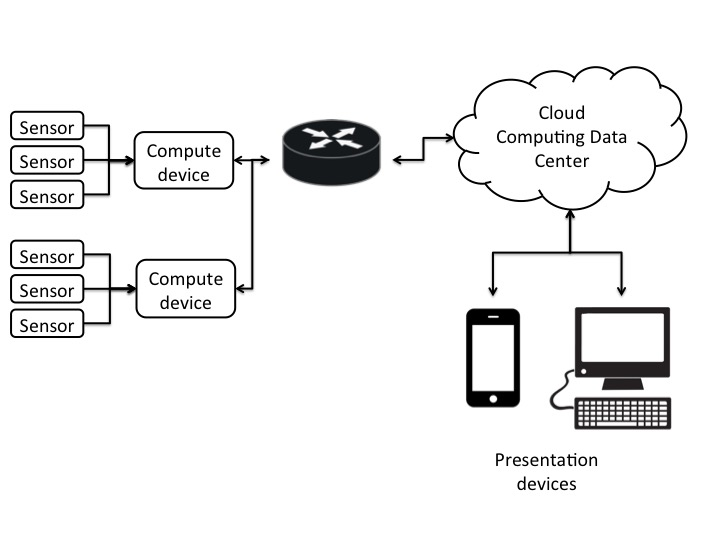
\includegraphics[width=0.75\textwidth]{images/IoT_diagram.jpg}
\caption{IoT full diagram }
\label{fig:1.1}
\end{figure}

Like many booming areas of technology, the internet of things revolution is
plagued by a lack of industry standards. As you can imagine there are thousands
of computing devices and sensors from different vendors that appear on the
market  every day , each one with his unique way to send  or store their data
in their centralized cloud computing centers.

Right now exist two main projects that are compiling to establish standards for
the IoT communications: 

\begin{itemize}
\item Open Interconnect Consortium (OIC): OIC is an industry group whose stated 
mission is to develop standards and certification for devices involved in the 
Internet of Things based around CoAP. OIC was created in July 2014 by Intel, 
Broadcom, and Samsung Electronics.\cite{OIC}

\item AllJoyn : AllJoyn is an open, universal, secure and programmable software 
connectivity and services framework that enables companies and enterprises to 
create inter-operable products that can discover, connect and interact directly 
with other AllJoyn-enabled products. \cite{AllJoyn}
\end{itemize}


Both standards try to solve a simple problem. Imagine you have smart light bulbs
in your house, all of them a device of your IoT network at home. What happened
if one them burns? You go and buy one but then you remember that all your
light bulbs at home are brand A and at the store there are only brand B
light bulbs. It should be possible to bring your any brand of light bulbs and
still work with the rest of the devices of your network. This will be possible
with communications standards among the industry.These two efforts are fighting
each other to generate these kind of standards in IoT communications. Which one
is the best ? maybe is too soon to have a winner, but in less than a decade
this question might be answered. 

In the meantime the Internet of Things revolution is here wetter we like it or
not. We live in houses with Computers insides our air conditions televisions
and cars; many of them connected to the internet. But as we have seen there are
parts that are being missing. Despite the efforts to develop standard network
protocols for IoT systems there is no effort to make the IoT systems analyze
their data among each others instead of send  all the data to Cloud Data centers
to be analyzed. This could be a problem in short future cause as we have seen
before the solution is not to add another server (specially when you have space
and economic constrains)


\section{Problem Definition}
\noindent

In order to understand the severity of the problem we have to understand the
magnitude of it, we have to understand that the rise of the internet of things
is real.  According to a study by the International Data Corporation (IDC)
\cite{IDC}, a market research analysis and advisory firm specialized in
information technology estimate the number of IoT devices is approaching  200
billion. And the number of sensors that track, monitor, or feed data to those
things is already more than 50 billion, with scientists talking about
trillion-sensor networks within 10 years. Of course, not all of those 200
billion things are actually wired and communicating on the Internet, but some
20 billion are. And, by 2020, this number will grow by 50\% to 30 billion
connected devices.\cite{EMC1}

But the rise of the internet of things means the rise of data. Imagine for a
moment that the 20 billion of devices try to send 1 Kilo Byte of data to the
centralized servers, this will create so much traffic that might be similar to
a security attack, collapsing the centralized data centers. One could imagine
that this is not a problem, that we might be exaggerating; but as we saw there
are actual problems like the one Virgin Atlantic airline has.

In 2014 the Boeing 787 aircraft ordered by Virgin Atlantic for delivery
dramatically increase the volume of data the airline will need to deal with
(half terabyte in a transatlantic flight). \cite{Finnegan} Because they can't
handle that much terabytes of data everyday coming from various airplanes they
are looking for cloud base solutions inside the airplanes. Now consider that
the space in an airplane is limited and expensive, moreover the electric
energy. A cloud base solution (adding servers inside the airplane) will require
both space and space and electric energy.

Besides that, the power consumption of these  IoT's Cloud Data Centers is a key
part to considerate. If current trends continue, a petaflop system will require 
100 megawatts to manage the IoT data \cite {Xizhou} (imagine that in an airplane)

The rise of IoT will lead to an explosion in the volume of data collected,
transmitted and processed.This will require novel and optimized solutions.  How
can we make the IoT networks self sustainable? Make them solve their own
compute problems without the need to send millions of data to the cloud data
centers?. How can we know when is really necessary to send the data to the cloud
data centers because the number of IoT systems is not efficient ( in terms of
energy and performance)? What kind of applications are good candidates for
these kind of solution? All these questions will be addressed in this work. 

\section{General Objective}
\noindent

The main objective is to find the maximum number of low ultra-low-voltage
microprocessors platforms that provides the maximum level of energy efficiency.

After finding this information for commons benchmarks it will be easy for the
industry of IoT systems to determine if their applications can take advantage
of communicate their IoT devices to process their own data instead of sending
the information to a data centers.

\section{Hypothesis}
\noindent

We are confident that with the current technology is possible to generate a
distributed system of of ultra-low-voltage microprocessors platforms (core
systems of the IoT devices). The part that we are concern is determine the
breaking point where is better to send the data to the cloud data centers. How
many systems is the maximum that these kind of network could support and still
being a good option in terms of energy efficiency?

In computing, performance per watt is a measure of the energy efficiency of a
particular computer architecture or computer hardware. Literally, it measures
the rate of computation that can be delivered by a computer for every watt of
power consumed.\cite{Burd} 


\begin{equation}
    Energy Efficiency = \dfrac {Performance}{Watts}
\end{equation}

We believe that the energy efficiency in an embedded cluster will have is the
behavior of the  figure~\ref{fig:1.2}. in the beginning the increment of the
number of nodes in our network will increment the performance (the top part of
the equation), but as the same time it increase the amount of watts will
increase making the energy efficiency flat at some point (if the lower part of
the equation increase the equation tends to decrease)


\begin{figure}[H]
\centering
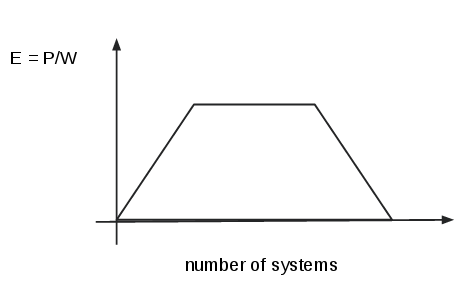
\includegraphics[width=0.75\textwidth]{images/graph_1.png}
\caption{Hypothesis of energy efficiency behavior in embedded cluster}
\label{fig:1.2}
\end{figure}

After finding these curves for command benchmarks it will be easy for the
industry of IoT systems to determine if their applications can take advantage
of communicate their IoT devices among each others instead of sending the
information to their data centers.


\section{Methodology}
\noindent

Recent researches \cite{Saldana} \cite{Gallego} \cite{McMahon} \cite{Liu} are 
showing an increasing interest in the topic.  All these research always talk
about the lack of three parts: 

\begin{itemize}
\item A low-voltage microprocessors platform with enough compute power
\item An operating system for Distributed System
\item A light communication protocol to distribute the workload among the
embedded platforms
\end{itemize}

The way we are going to address this will be:


\begin{itemize}

\item Chose the right embedded platform: There are dozens of embedded and IoT
platforms, this is why is necessary to make a deep analysis and choose the best
platform that feed our needs. (taking into consideration that sometimes the
systems might have heterogeneous platforms)

\item Chose the right communication and compute protocol: There are different
kinds of distributed compute protocols. Part of this investigation is to detect
the most reliable and suitable for our needs.

\item Chose the right Operating System for the system. Once we have selected
the appropriate embedded platforms, another variable in this investigation is
the number of Operating Systems. Either if is a micro kernel or a monolithic
kernel architecture there are more than a dozen of solutions to use.

\item Crate embedded clusters to measure energy efficiency. Once we have find
the best configuration (Hardware + Operating System + Communication Protocol )
in terms of energy efficiency , we can start to create a cluster of embedded
systems.

\item Release all the improvements and disagreements found Open Source and
public. All the improvements made into any technology (operating systems or
communication protocols) will be published with an open source license.

\item Implement solution on real application ( greenhouse ). In order to test
or hypothesis in a real application we will implement it on a real greenhouse.
Proving that the solution give an embedded system the power of reliability and
availability without the need of external and expensive servers 
\end{itemize}


\clearpage

  %Empieza configuracion de capitulo
\setstretch{1.0}
\titleformat{\chapter}[block]{\Large\bfseries}{CHAPTER \Huge\thechapter\vspace{25 pt}}{0 pt}{\\\fontsize{26}{36}\selectfont}
\titlespacing{\chapter}{0 pt}{30 pt}{50 pt}[0 pt]
\titleformat{\section}{\Large\bfseries}{\thesection}{0 pt}{\hspace{30 pt}}
\titleformat{\subsection}{\large\bfseries}{\thesubsection}{0 pt}{\hspace{30 pt}}
\pagestyle{fancy}
\fancyhead[LO,LE]{\footnotesize\textit{\leftmark}}
\fancyhead[RO,RE]{\thepage}
\fancyfoot[CO,CE]{}
%Termina configuracion de capitulo

\chapter{Objectives} %Cambia Marco Te'orico al nombre de tu capitulo
\setstretch{1.5} %Regresa el interlineado a 1.5

\normalsize

\section{General Objective}
\noindent

The main objective is to present a methodlogy to crate a self sustainable
network of ultra-low-voltage microprocessors platforms. It means the embedded 
devices interconected could process their own workload without the need of an 
external compute system

The purpose of this methodology is to give an experienced IoT  developer 
enough information to replicate the study. At the same time it offers the theoretical 
underpinning for understanding which method, set of methods, or so-called “best 
practices” can be applied an specific case


\section{Justification}
\noindent

The development of wireless sensor networks has reached a point where each 
individual node of a network may store and deliver a massive amount of 
(sensor-based) information at once or over time. Right now the total amount of 
user data (data payload) to be stored or processed doubles every two years. Consequently,
data will become a problem for traditional data aggregation strategies 
traffic-wise as well as with regard to energy efficiency. 

These problems start to be relevant in current industries. Such is the case of 
the Aircraft industry. On March of 2013 Virgin Atlantic was preparing for a 
significant increase in data as it embraces the internet of things, with a new fleet of highly 
connected planes each expected to create over half a terabyte of data per flight.

Speaking to the Computerworld UK magazine at the Economist Technology Frontiers 2103 event, Virgin 
Atlantic IT director David Bulman said that the airline company was expecting an 
"explosion" of information generated from a growing number of sources, from 
employees and customers to cargo containers and planes.

In particular, the introduction of Boeing 787 aircraft ordered by Virgin 
Atlantic for delivery in 2014  was expected to dramatically increase the volume 
of data the airline will need to deal with.

From the interview Bulman hightlight their current problems: 

\say{The challenge is what do you do with that amount of data when you are getting 
terabytes of data a day off your various airplanes? We are getting to the stage 
right now where we cannot deal with that much}

He added: 

\say{If you are talking that level of data you can't just chuck ten disks 
into your data centre anymore, you have to look at cloud based solutions and how 
you can store data.}

As we can see the lack of standard solutions for self sustainable networks is 
creating real problems among the industry


\clearpage

	%Empieza configuracion de capitulo
\setstretch{1.0}
\titleformat{\chapter}[block]{\Large\bfseries}{CHAPTER \Huge\thechapter\vspace{25 pt}}{0 pt}{\\\fontsize{26}{36}\selectfont}
\titlespacing{\chapter}{0 pt}{30 pt}{50 pt}[0 pt]
\titleformat{\section}{\Large\bfseries}{\thesection}{0 pt}{\hspace{30 pt}}
\titleformat{\subsection}{\large\bfseries}{\thesubsection}{0 pt}{\hspace{30 pt}}
\pagestyle{fancy}
\fancyhead[LO,LE]{\footnotesize\emph{\leftmark}}
\fancyhead[RO,RE]{\thepage}
\fancyfoot[CO,CE]{}
\setcounter{secnumdepth}{5}
%Termina configuracion de capitulo

\chapter{Theoretical Framework}
\setstretch{1.5} %Regresa el interlineado a 1.5

\normalsize
\noindent

This chapter will describe some basic topics to fully understand further
experiments and why we decided to do them. We will try to cover as much of the
topics needed to fully understand the problem and the proposed solution.
However will not cover deep topics as Operating Systems architecture nor
parallel programming concepts.


\section{The need of parallel computing}
\noindent

Based on all the current advantages we have today ( smart-phones, tablets,
smart cars and more ) thanks to the power the computer has achieve, one coudl
think that the computer design has been evolving like any other technology.
However the progress in the computer architectures has been much less
consistent.  During the first 25 years of electronic computers \footnote{since
1951 with the introduction of UNIVAC} the improvement in performance increase
about 25\% per year \cite{Hennessy}. 


It was until the late 1970s  when the world saw the emergence of the
microprocessor. This major change in technology aloud the industry to improve
the scalability of the integrated circuits. After the introduction of the
microprocessor the improvement in performance per year in the computer
architectures increase to 35\% \cite{Hennessy}   

But the advances in computer architecture were not the only one responsible for
this great increase in performance. In particular two significant changes make
the life of users easy. First, the elimination of assembly language with the
invention of the C programing language, a much more easy to read and use
programing language. The C programing language give the user the power to
handle memory and peripheral devices in a much more friendly way. Second, the
creation of standardized and free  operating systems, such as UNIX and its
clone, Linux. These operating systems lowered the cost and risk of bringing out
to the market brand new products

In the decade of 1980 the idea of making the microprocessor architecture faster
starts to take form with the RISC (Reduced Instruction Set Computer)
architecture .  The RISC microprocessor is designed to perform a smaller number
of types of computer instructions so that it can operate at a higher speed. 
The RISC-based computers raised the performance bar. This architecture
principle in conjunction with the transistor size reduction ( allowing to have
much more compute power in less space) led to 16 years of sustained growth in
performance at an annual rate of over 50i\%

It was around the years 2003 to 2005 that a dramatic change seized the
semiconductor industry and the manufactures of processors. The increasing of
computing performance in processors, based on simply screwing up the clock
frequency, could not longer be sustainable. The problem with increasing the
frequency in the microprocessor is that the heat in the chip also increase.  In
fact in 2004 Intel canceled its high-performance projects declaring that
\textit{the road to higher performance would be via multiple processors per
chip rather than via faster uniprocessors}

The answer of the industry to that development, in order to still meet Moore's
law \footnote{the number of transistors in a dense integrated circuit doubles
approximately every two years.}, was the shifting to real parallelism by
doubling the number of processors on one chip die. This was the birth of the
multi-core area. 

With the multi core are there was a need to change the paradigm in programing
languages. The programs that had been designed before this change were mostly a
sequence of instructions to calculate or control a system. With the multi core
architecture came the birth of the parallel programing. The parallel programing
codes are properly designed to take advantage of parallelism can execute faster 

However not all the problems can be solved using parallel programing
techniques. In order to use this approach the problem need to be represented as
a collection of simultaneously executing tasks. This is especially the case in
many areas of scientific, mathematical, and artificial intelligence
programming. After the birth of the parallel computing all these technology
areas had a growth never seen before

At the same time that the parallel computing came many other technologies was
already established: the emergence of the Internet and the World Wide Web, the
popularity of cell-phones since 2000 and the broadly use of laptops. According
to \cite{Hennessy} all  these technologies have led to three different computing
markets: desktop computing, servers and embedded. 

The problem we have will require a deep understanding of the server and
embedded components. So far we have seen why the world needed the parallel
computing as well as the evolution of the computer architecture that aloud us
to arrive here.

\section{Servers Systems}
\noindent

The growth of mobile personal computers coupled with the popularity of
cellphones changed the role of servers to provide scale and reliable storage
and computing services. The emerge of faster Internet connections accelerate
the demand of web-based services make the transition of compute power from
personal computers to servers

But the fact of provide storage and compute services to thousands of users came
with a lot of responsibility. A failure of server systems is far more
catastrophic than failure of a single desktop, since these servers must operate
seven days a week, 24 hours a day Is because of this that reliability is a key
factor for a server system.

A second key feature of server systems is scalability. With the number of users
changing every minute the ability to scale up the computing capacity
in server is crucial. A web sale page should be able to response every as well
as during a peak hour for Christmas shoppings.

The third key feature is throughput. Servers are designed for efficient
throughput \footnote{Throughput is a measure of how many units of information a
system can process in a given amount of time} in terms of transactions per
minute or Web pages served per second. From the user perspective point of view
is the speed of response.

Is because of these three factors that the server technology has change. The
cloud era is dominating the computing and storage services.  According to \cite
{Farhan} \textit{"Cloud computing is set of resources and services offered
through the Internet"}. Cloud services are delivered from data centers located
around the world.  Cloud computing provides virtual resources via internet. The
best example of cloud computing is the streaming video services. Nowadays users
can stream online videos  at any time, without the need to storage the movie at
home. All the resources and infrastructure are provided upon request. With this
the scalability, reliability and manageability are guaranteed by the compute
service providers. 

\section{Embedded Systems}
\noindent

The birth of multi core architecture not only provide the servers with much
more compute power it also break the paradigm of use low compute power
microprocessors for embedded platforms. Now it was possible to have more
compute power with less frequency. Thanks to this radical change there has been
a rapid evolution of the compute and multimedia capabilities of embedded
systems. At the point where have more computer power in our cellphones than all
of NASA back in 1969 \cite{Michio}

According to \cite{Hallinan} \textit{"An embedded system is a special-purpose
system in which the computer is completely encapsulated by the device it
controls"} Unlike a general-purpose computer, such as a personal computer, an
embedded system performs pre-defined tasks, usually with very specific
requirements. Examples of these are:microwaves, washing machines, printers, and
GPS (Global Positioning System) systems. All those electronic gadgets that
started to emerge 15 years ago \cite{Nur}.

The variety of the embedded applications requires at the widest spread
of processing power and cost. They include 8-bit and 16-bit processors that may
cost few cents, 32-bit microprocessors that execute 100 million instructions
per second and cost less than few dollars, and high-end processors for the
newest video games or network switches that cost at least 100 dollars and can
execute a billion instructions per second.\cite{Hennessy}

Since its origins, the RISC technology has been the default technology in the
more complex embedded architectures. Due to the fact that The RISC
microprocessor is designed to perform a smaller number of types of computer
instructions the power consumption can be much more lower. This architecture
concept was fine until the new embedded applications such as smart-phones,
tablets and smart TVs start to appear.

The increment in the complexity of the new embedded applications started to
require more specialized integrated circuits that could help the microprocessor
with all these task in parallel . Wireless networking cards, Digital Signal
Processors, I/O controls, peripherals ( such as USB controllers ) and analog
interfaces (including ADCs and DACs) became part of the requirements of an
embedded platform. Soon the architecture designers realize that the
communication with all these components decrease the performance and increase
the power consumption. Is because of this that the last decade saw the emerge
of the System of a Chip (SOC)  embedded platforms. 

The SoC is an integrated circuit with all these components into a single chip.
With all these components in the same integrated circuit the communication
latency and power consumption was reduced considerably. Since the birth of the
SoC architecture the variety of gadgets using embedded platforms has increasing
every year.  Every year some basic goals are pursued:  increment in compute
performance, cost,  size and power density reduction.

\section{Embedded Linux Systems}

Computers are everywhere, we already know that computers aren't just on our
desktops, they are in our kitchens  and increasingly in our living rooms
holding our music collections. They're also in our microwave ovens, our regular
ovens, our cellphones, and our portable digital music players.

Until not too long time ago, embedded systems were not very powerful, and they
ran special-purpose, proprietary operating systems that were very different
from industry-standard ones. (Plus, they were much harder to develop for.)
Today, embedded computers are as powerful as, if not more than, a modern home
computer. (Consider the high-end gaming consoles, for example.)

Along with this power comes the capability to run a full-fledged operating
system such as Linux. Using a system such as Linux for an embedded product
makes a lot of sense. It was thanks to the free operating system UNIX and its
easy user experience, that the number of users of computer increase in the
early birth of personal computers. The evolution of UNIX, Linux, has been one
of the most sustainable projects in the history of computing. The fact that a
large community of developers find novel ways to improve performance and fix
critical failures every day are the key to think that Linux could be the best
solution in terms of sustainability for embedded platforms.

According to \cite{Hallinan} there are multiple reasons why Linux is the best choise
for current embedded platforms 

\begin{enumerate}
\item Linux supports a huge variety of applications and networking protocols.
Linux is scalable, from small consumer-oriented devices to large, heavy-iron,
carrier-class switches and routers.
\item Linux can be deployed without the royalties required by traditional proprietary
embedded operating systems.
\item Linux has attracted a huge number of active developers, enabling rapid support
of new hardware architectures, platforms, and devices.
\item An increasing number of hardware and software vendors, including virtually all
the top-tier manufacturers and ISVs, now support Linux.
\end{enumerate}

For these and other reasons, we are seeing an accelerated adoption rate of
Linux in many common embedded platforms. With the birth of the SoC systems the
use of these complete operating systems was necessary due to the need of handle
process concurrency, memory management and network connectivity.

Although the idea of using Linux as main operating system for embedded platform
was easy in reality it was not. With too many configure options and no standard
methodologies or templates to reuse the process to customize a Linux Operating
System for embedded platforms became a complex work for software engineers.
Every new embedded company create his own version ( according to his needs
without any standards) with very low maintainability and robustness. In 2010
there was a change in the industry of embedded systems, the announce of a
project to solve these kind of problems: The Yocto project.

The Yocto Project is an open source collaboration project that provides
templates, tools and methods to help you create custom Linux-based systems for
embedded products regardless of the hardware architecture\cite{yocto-project}.
It was founded in 2010 as a collaboration among many hardware manufacturers,
open-source operating systems vendors, and electronics companies to bring some
order to the chaos of embedded Linux development.\cite{Leppakoski}

The Yocto project  is a  complete embedded Linux development environment with
tools, meta-data, and documentation. The free tools are easy to get started
with, powerful to work with (including emulation environments, debuggers, an
Application Toolkit Generator, etc.) and they allow projects to be carried
forward over time without causing you to loose optimizations and investments
made during the project's prototype phase. The Yocto Project fosters community
adoption of this open source technology allowing its users to focus on their
specific product features and development.

The Yocto Project through the Poky build tool provides an open source
development environment (figure~\ref{fig:3.1})  targeting the ARM, MIPS,
Power-PC and x86 architectures for a variety of platforms including x86-64 and
emulated ones.  You can use components from the Yocto Project to design,
develop, build, debug, simulate, and test the complete software stack using
Linux, the X Window System, GNOME Mobile-based application frameworks, and Qt
frameworks. 

\begin{figure}[H]
\centering
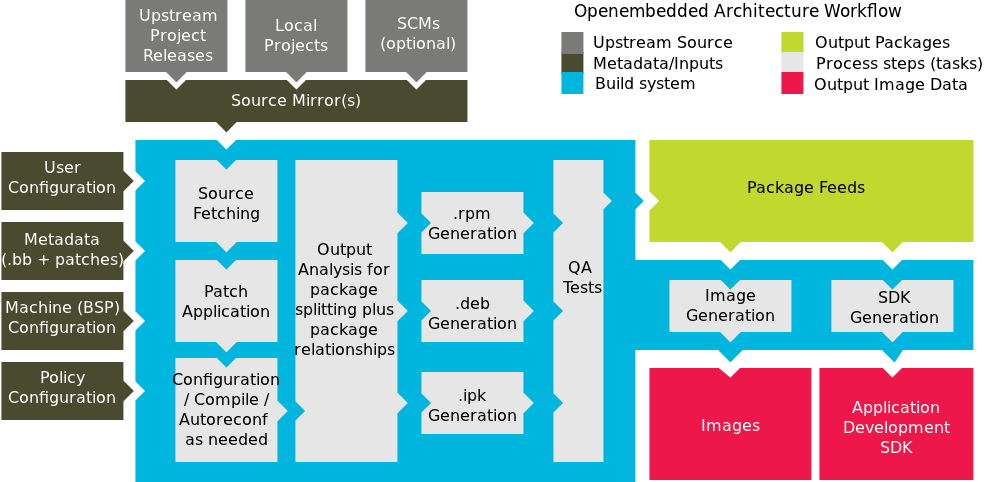
\includegraphics[width=0.75\textwidth]{images/yocto-environment.png}
\caption{The Yocto project development environment}
\label{fig:3.2}
\end{figure}

As we can see the Yocto project will play an important role in the IoT world.
If we want to develop a solution standard for multiple platforms we might adapt
it for the Yocto project. If we do this our solution will be deployable into
multiple IoT devices due to the bast amount of platforms ( sensors and
processing devices ) that use the Yocto project everyday.

\section{Ubiquitous Computing and IoT}
\noindent

The combination of all these factors (the cost, size, and power density
reduction) in combination with the increase in computing power and connectivity
has caused the computing technology to evolve into ubiquitous computing.
According to Mark \cite{Mark}, ubiquitous computing is \textit{"the method of
enhancing computer use by making many computers available throughout the
physical environment, but making them effectively invisible to the user"}. This
mean that the computing power is available anywhere and at any time


According to \cite{Nur} currently we are moving from ubiquitous computing into
advanced ubiquitous computing. An advanced ubiquitous computing is an extension
of ubiquitous environment that improve connectivity between devices. The major
characteristics of this environment can be stated as follows: 

\begin{itemize}
\item Large number of heterogeneous devices
\item New communication technology
\end{itemize}

This  devices include devices such as notebook computers, tablets, smartphones
and wearable computers. Most of these devices operate under many different
operating systems. New communication technology 4G , 5G and the introduction of
IPv6 provides bigger and faster of data bandwidth and much better than 3G in
data performance.

One of the most accurate definitions of the IoT is the one given by
\cite{Bahga} where it mentions that "Internet of Things refers to physical and
virtual objects that have unique identities and are connected to the internet
to facilitate intelligent applications [...] smarter". The IoT enables the
interconnection via the Internet of computing devices embedded in everyday
objects, enabling them to send and receive data. As you can see the differences
with traditional embedded systems are the internet connectivity and less power
consumption.  IoT systems must always be connected to the internet which
require a lower power consumption

The IoT computing is new era of computing technology that we have to explore.In
collaboration with the cloud computing the capability to have smart
applications in multiple scenarios is imminent. In the middle of all these
technology an invisible architecture design was established , transparent for
the user , but always there sustaining the reliability, scalability and
reliability of the systems, it was the distributed architecture systems.

\section{Distributed Systems}
\noindent

We define a distributed system as one in which hardware or software components
located at networked computers communicate and coordinate their actions only by
passing messages. This simple definition covers the entire range of systems in
which networked computers can usefully be deployed.

Computers that are connected by a network may be spatially separated by any
distance. They may be on separate continents, in the same building or in the
same room. Our definition of distributed systems has the following significant
consequences:


\begin{enumerate}

\item \textbf{Concurrency:}
In a network of computers, concurrent program execution is the norm. I can
do my work on my computer while you do your work on yours, sharing resources
such as web pages or files when necessary. The capacity of the system to handle
shared resources can be increased by adding more resources (for example.
computers) to the network.

\item \textbf{No global clock:}
When programs need to cooperate they coordinate their actions
by exchanging messages. Close coordination often depends on a shared idea of
the time at which the programs actions occur. But it turns out that there are
limits to the accuracy with which the computers in a network can synchronize
their clocks there is no single global notion of the correct time. This is a
direct consequence of the fact that the only communication is by sending
messages through a network.

\item \textbf{Independent failures:}
All computer systems can fail, and it is the
responsibility of system designers to plan for the consequences of possible
failures. Distributed systems can fail in new ways. Faults in the network
result in the isolation of the computers that are connected to it, but that
doesn't mean that they stop running. In fact, the programs on them may not be
able to detect whether the network has failed or has become unusually slow.
Similarly, the failure of a computer, or the unexpected termination of a
program somewhere in the system (a crash), is not immediately made known to the
other components with which it communicates. Each component of the system can
fail independently, leaving the others still running.

\end{enumerate}


Each one these characteristics is also present in a modern IoT system. As we can
see in (figure~\ref{fig:3.1}). As we can see these three characteristics of a
distributed system are also present in an IoT system. 

\begin{figure}[H]
\centering
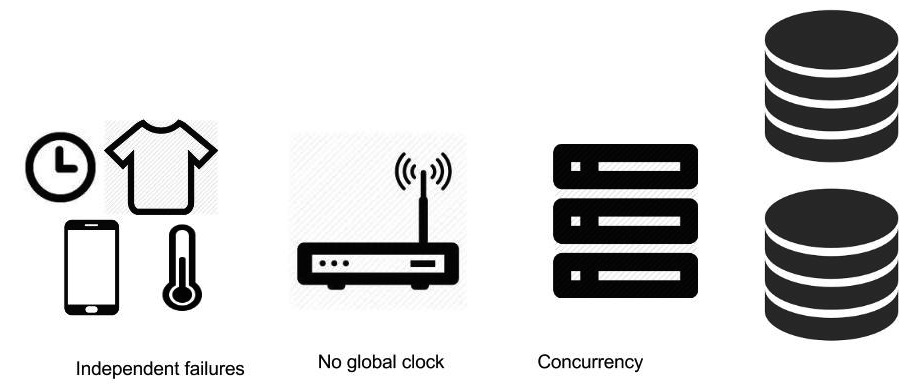
\includegraphics[width=0.75\textwidth]{images/IoT_distributed.jpg}
\caption{IoT system as a distributed system}
\label{fig:3.1}
\end{figure}


\begin{enumerate}
\item \textbf{Concurrency}
In an IoT system there are multiple systems trying to use the same resource.
For example all the IoT devices are trying to access the same data base or the
even the same access's point. All of them are fighting for similar resources , a
good IoT design need to schedule the use of the limited resources in an efficient
way.

\item \textbf{No global clock}
None of the systems in an IoT network (either sensors or processing devices)
have the same clock. They have to use a message base mechanism to communicate
each other. 

\item \textbf{Independent failures}
In a regular IoT network multiple systems could fail (either sensors,
processing devices or one of the data centers) and despite of that all the
others should keep working without any problem. 

All these characteristics enforce the idea that the nature of an IoT system is
being treated as a distributed system. With this main idea is much more simple
to adapt the solutions of the distributed systems into our embedded distributed
system.

\end{enumerate}

\section{Message-Passing Interface Library}
\noindent

The Message-Passing Interface (MPI) is a message-passing library interface
specification. MPI addresses primarily the message-passing parallel programming
model, in which data is moved from the address space of one process to that of
another process through cooperative operations on each process

MPI is not a language, and all MPI operations are expressed as functions,
subroutines, or methods, according to the appropriate language bindings which,
for C and FORTRAN, are part of the MPI standard. The standard has been defined
through an open process by a community of parallel computing vendors, computer
scientists, and application developers

Despite all the advantages that MPI has it is not widely used in embedded
systems (due to the fact that these abstraction layers require extensive
system resources with comprehensive operating systems support, which may not be
available to an embedded platform) but as we have seen this is now possible. We
do have a powerful ultra-low-voltage microprocessor platform
\cite{minnowboard} and we do have robust distributed operating systems running on
those platforms. The missing part now is to set up the message passing library
interface on the top of all the system. 

Recent researches \cite{Saldana} \cite{Gallego} \cite{McMahon} describe
proof-of-concept MPI implementations targeting embedded systems, showing an
increasing interest in the topic. However none of theme has been implemented in
the current embedded Linux operating systems (like the ones generated with
Yocto project\cite{yocto-project}) nor the standard Linux (like
Fedora\cite{fedora})

After a quick review on the current operating systems we found that the only
one missing the MPI implementation was actually the Yocto project.


\begin{center}
\begin{tabular}{ | l | r |}
    \hline
    Operating System & MPI library  \\ \hline
    Fedoras & Implemented  \\ \hline
    Clear Linux for Intel Architecture & Implemented  \\ \hline
    OS generated with Yocto project & Not Implemented  \\ \hline
\end{tabular}
\captionof{table}{Linux OS supported MPI implementation on MinnowBoard MAX}
\label{tab:4.2}
\end{center}


\section{Performance and Power Efficiency}

\noindent

The meaning of performance may be different according to the application.
The user of a desktop computer may say a computer is faster when a program runs in less
time, while an Amazon.com administrator may say a computer is faster when it
completes more transactions per hour. The computer user is interested in 
reducing response time (the time between the start and the completion of an 
event) \cite{Hennessy} also referred to as execution time. The administrator of a large data 
processing center may be interested in increasing throughput (the total amount 
of work done in a given time.) \cite{Hennessy}. 

According to \cite{Hennessy} in comparing design alternatives, we often want to
relate the performance of two different computers, say, X and Y. The phrase ''X
is faster than Y'' is used here to mean that the response time or execution
time is lower on X than on Y for the given task. In particular, ''X is n times
faster than ''  will mean \ref{eq:2}:

\begin{equation}\label{eq:2}
n = \frac{Execution time x}{Execution time y}
\end{equation}

Since execution time is the reciprocal of performance, the following
relationship holds in formula \ref{eq:3}:

\begin{equation}\label{eq:3}
n = \frac{Execution time x}{Execution time y} = \frac{\frac{1}{Performance
x}}{\frac{1}{Performance y}} = \frac{Performnace x}{Performance y}
\end{equation}

Another metric to considerate is the throughput. According to \cite{Hennessy}
\textit{"the throughput of X is 1.3 times higher than Y signifies that the
number of tasks completed per unit time on computer X is 1.3 times the number
completed on Y"} . Unfortunately, time is not always the metric quoted in
comparing the performance of computers. The only consistent and reliable
measure of performance is the execution time of real programs. 

The most straightforward definition of execution time is given by
\cite{Hennessy} \textit{"it is called wall-clock time, response time, or elapsed
time, which is the latency to complete a task, including disk accesses, memory
accesses, input/output activities, operating system over head everything"}.
Even in current multi processors world this is transparent for the users,  the
response time seen by the user is the elapsed time of the program, not the CPU
time.

But in parallel programing the performance metric is measure in a different
way.  With the current compute power of compute devices is possible to create a
cluster of computers. All of the inter-connected in a network that provides the
maximum level of performance with the less amount of power consumption. This
characteristic is determined by the power efficiency of the network. The power
efficiency is quantified by performance per watt \cite{Jun}

The critical part is to determine the breaking point where is better to send
the data to the cloud data centers. How many systems is the maximum that these
kind of network could support and still being a good option in terms of energy
efficiency

The development of metrics to evaluate energy efficiency on the basis of
performance and power models is described in \cite{Dong}. According to
\cite{Dong} the formula for computing the theoretical maximum speedup (or
performance) achievable through parallelization is \ref{eq:4}

\begin{equation}\label{eq:4}
Perf = \frac{1}{(1 - f) + \frac{f}{n}}
\end{equation}

Where \textit{n} is the number of processors,  \textit{f} is the fraction of
computation that programmers can parallelize  ( form 0 to 1 ) . To model the
power consumption for a \textit{P} many-core processor, \cite{Dong} introduce a
new variable, \textit{k}, to represent the fraction of power the processor
consumes in idle state \ref{eq:5}. 

\begin{equation}\label{eq:5}
\frac{Perf}{W} = \frac{1}{(1 + (n -1 ) k (1 - f))}
\end{equation}

In \cite{Dong} their analysis clearly demonstrates that a symmetric many-core
processor can easily  lose its energy efficiency as the number of cores
increases. To achieve the  best possible energy efficiency, their  work
suggests a many-core alternative, featuring many small, energy-efficient cores
integrated with a full-blown processor. They also show that by knowing the
amount of parallelism available in an application prior to execution, is
possible to  find the optimal number of active cores for maximizing performance
for a given cooling capacity and energy in a system

\section{Benchmarks}

In computer science a benchmark is a test to measure the performance of
multiple applications over the same standard way. The best choice of benchmarks
to measure performance are real applications. Due to the complexity of the
current applications the software engineers are making small versions of them
to be used as benchmarks. According to \cite{Hennessy} there are three kind of
them: 

\begin{itemize}
\item kernels, which are small, key pieces of real applications.
\item Toy programs, which are 100-line programs from beginning programming
assignments.
\item Synthetic benchmarks, which are fake programs invented to try to match the
profile and behavior of real applications.
\end{itemize}

One of the most successful attempts to create standardized benchmark
application suites has been the SPEC (Standard Performance Evaluation
Corporation), which had its roots in the late 1980s efforts to deliver better
benchmarks for workstations\cite{Hennessy}. All the SPEC benchmark suites and
their results are found at www.spec.org.

In terms of parallel and distributed computing (MPI) there are already numerous
MPI benchmark suites available , such as Mpptest \cite{Gropp}, MP-Bench
\cite{Calderon} and  SKaMPI \cite{Hoefler} are examples of them. Many of give
timing results for message passing routines. This is useful for performance
modelling and analysis of parallel programs, as well as for understanding the
performance of parallel machines. Based on the results in \cite{Grove} we
decided to use MPIbench as our default benchmark testing framework. MPIbench is
a benchmark that allows to evaluate the performance of MPI on MPP's and cluster
of workstations. MPIbench tests different MPI calls.

\subsection{MPIbench}
\noindent

The benchmarks we are going to run are the MPIbench (or MPbench) version 4
\cite{mpibench}.This is a program to measure the performance of some critical
MPI functions. By critical we mean that the behavior of these functions can
dominate the run time of a distributed application.

MPIBench currently tests eight different MPI calls. The following functions are
measured:

\begin{itemize}
    \item Bandwidth (BB/second)
    \item Gap Time (time to launch a message and continue) (Us)
    \item Roundtrip or 2 * Latency (transactions/second)
    \item Asynchronous Bidirectional bandwidth (KB/second)
    \item Broadcast (KB/second)
    \item Sum reduction (KB/second)
    \item All-reduce (KB/second)
    \item AlltoAll (KB/second)
\end{itemize}



All tests are timed in the following manner.

\begin{itemize}
    \item Set up the test.
    \item Start the timer.
    \item Loop of operations over the message size as a power of two and the
iteration count.
    \item Verify that those operations have completed.
    \item Stop the timer.
    \item Compute the appropriate metric
\end{itemize}

By default, MPIBench measures messages from 4 bytes to 216 bytes, in powers of
two for 100 iterations. Each test is run a single time before testing to allow
for cache setup and routing. The cache is then flushed before each repetition
and before each new message size is tested. The cache is not flushed however
between iterations on the same message size, which are averaged

We will describe each one of the tests in order to understand the experiments.


\subsubsection{Bandwidth}

MPIBench measures bandwidth with a doubly nested loop. The outer loop varies the
message size, and the inner loop measures the send operation over the
iteration count. After the iteration count is reached, the slave process
acknowledges the data it has received by sending a four byte message back to
the master. The master's pseudo code for this test is as follows:

\begin{minipage}{\textwidth}
\end{minipage}

\begin{minipage}{\linewidth}
\begin{lstlisting}[frame=single,numbers=left]
do over all message sizes 
    start timer
    do over iteration count 
        send(message size) 
        recv (4)
    stop timer
\end{lstlisting}
\end{minipage}

The slaves' pseudo code is as follows:

\begin{minipage}{\textwidth}
\end{minipage}

\begin{minipage}{\textwidth}
\begin{lstlisting}[frame=single,numbers=left]
do over all message sizes 
    start timer
    do over iteration count 
        recv(message size) 
        send(4)
    stop timer
\end{lstlisting}
 \end{minipage}

\subsubsection{Bidirectional Bandwidth}

MPIBench measures bidirectional bandwidth with a doubly nested loop. The outer
loop varies the message size, and the inner loop measures the send operation
over the iteration count. Both processes execute a non-blocking receive, then a
non-blocking send, and then a wait for each iteration. The next iteration is
prevented from proceeding until the previous one is finished by the MPLWaitall0
call, which will not allow execution to continue until both messages have been
completed.

The code for this test is as follows:
 
\begin{minipage}{\textwidth}
\end{minipage}

\begin{minipage}{\textwidth}
\begin{lstlisting}[frame=single,numbers=left]
 do over all message sizes
    start timer
    do over iteration count
        immediate (nonblocking) receive(message size)
        immediate (nonblocking) send(message size)
        wait until messages on both ends have been received
    stop timer
\end{lstlisting}
\end{minipage}

\subsubsection{Roundtrip}

Roundtrip times are measured in much the same way as bandwidth, except that,
the slave process, after receiving the message, echoes it back to the master.
This benchmark is often referred to as ping-pong. Here our metric is
transactions per second, which is a common metric for database and server
applications. No acknowledgment is needed with this test as it is implicit
given its semantics.

The master's pseudo code for this test is as follows:

\begin{minipage}{\textwidth}
\end{minipage}

\begin{minipage}{\textwidth}
\begin{lstlisting}[frame=single,numbers=left]
  do over all message sizes 
    start timer
    do over iteration count
        send(message size)
        recv(message size) 
        stop timer
\end{lstlisting}
\end{minipage}

The slaves' pseudo code is as follows:

\begin{minipage}{\textwidth}
\end{minipage}

\begin{minipage}{\textwidth}
\begin{lstlisting}[frame=single,numbers=left]
do over all message sizes 
    start timer
    do over iteration count
        recv(message size)
        send(message size)
    stop timer
\end{lstlisting}
\end{minipage}

\subsubsection{Application Latency}

Application latency is something relatively unique to MPBench. This benchmark
can properly be described as one that measures the time for an application
to issue a send and continue computing. This benchmark is the same as
bandwidth except that we do not acknowledge the data and we report our
results in units of time.

The master's pseudo code for this test is as follows:

\begin{minipage}{\textwidth}
\end{minipage}

\begin{minipage}{\textwidth}
\begin{lstlisting}[frame=single,numbers=left]
do over all message sizes 
    start timer
    do over iteration count 
        send(message size) 
    stop timer
\end{lstlisting}    
\end{minipage}

The slaves' pseudo code is as follows:

\begin{minipage}{\textwidth}
\end{minipage}

\begin{minipage}{\textwidth}
\begin{lstlisting}[frame=single,numbers=left]
   do over all message sizes 
        start timer
        do over iteration count 
            recv(message size) 
        stop timer
\end{lstlisting}
\end{minipage}

\subsubsection{Broadcast and Reduce}

Both of these benchmarks return the number of megabytes per second computed
from the iteration count and the length argument given to function call.

Here is the pseudo code for both the master and the slave:

\begin{minipage}{\textwidth}
\end{minipage}

\begin{minipage}{\textwidth}
\begin{lstlisting}[frame=single,numbers=left]
   do over all message sizes 
        start timer
        do over iteration count
            reduce or broadcast(message size)
        stop timer
\end{lstlisting}
\end{minipage}

\subsubsection{AllReduce}

AllReduce is a derivative of an all-to-all communication, where every
process has data for every other. While this operation could easily be
implemented with a reduce followed by a broadcast, that would be highly
inefficient for large message sizes. 

Here is the pseudo code for both the master and the slave:

\begin{minipage}{\textwidth}
\end{minipage}

\begin{minipage}{\textwidth}
\begin{lstlisting}[frame=single,numbers=left]
    do over all message sizes 
        start timer
        do over iteration count 
            allreduce(message size) 
        stop timer
\end{lstlisting}
\end{minipage}

\subsubsection{All-to-all}

MPBench measures a kind of round-robin communication among multiple
processes. The outer loop varies the message size, and the inner loop
measures the send operation over the iteration count. Each process sends a
message of the size of the total message size divided by the number of
processes to every other process.

The code for this test is as follows:

\begin{minipage}{\textwidth}
\end{minipage}

\begin{minipage}{\textwidth}
\begin{lstlisting}[frame=single,numbers=left]
    do over all message sizes 
        start timer
        do over iteration count 
            all-to-all(message size)
        stop timer
\end{lstlisting}
\end{minipage}

\clearpage

	%Empieza configuracion de capitulo
\setstretch{1.0}
\titleformat{\chapter}[block]{\Large\bfseries}{CAP'ITULO \Huge\thechapter\vspace{25 pt}}{0 pt}{\\\fontsize{26}{36}\selectfont}
\titlespacing{\chapter}{0 pt}{30 pt}{50 pt}[0 pt]
\titleformat{\section}{\Large\bfseries}{\thesection}{0 pt}{\hspace{30 pt}}
\titleformat{\subsection}{\large\bfseries}{\thesubsection}{0 pt}{\hspace{30 pt}}
\pagestyle{fancy}
\fancyhead[LO,LE]{\footnotesize\emph{\leftmark}}
\fancyhead[RO,RE]{\thepage}
\fancyfoot[CO,CE]{}
%Termina configuracion de capitulo

\chapter{Reglas de Presentaci'on} %Cambia al nombre de tu capitulo
\setstretch{1.5} %Regresa el interlineado a 1.5

\normalsize
\noindent
Este manual de tesis se basa, en parte, del estilo establecido por la Rector'ia de la Universidad Virtual (UV) del Sistema Tecnol'ogico de Monterrey \cite{Demo:manualUV} y publicado por la American Psychological Association (APA) \cite{Demo:APA,Demo:manualAPA}. Los alumnos de las maestr'ias de la EGIA (Escuela de Graduados en Ingenier'ia y Arquitectura) del ITESM Campus Guadalajara deben considerar que es imprescindible apegarse a las reglas de estilo que se presentan en este manual.

Las siguientes reglas de formato son aplicables a las maestr'ias ofrecidas por la EGIA. Aseg'urate de seguirlas minuciosamente. Este manual est'a escrito estrictamente de acuerdo a las reglas generales y particulares que se mencionan a continuaci'on, as'i que le sirve como modelo para escribir tanto su documento de anteproyecto de tesis, como su documento final.

\section{Reglas generales}
\noindent
\begin{enumerate}
	\item Imprime solamente en un lado de la p'agina.
	\item Usa sangr'ias para cada p'arrafo nuevo, a excepci'on del primer p'arrafo que sigue a un cap'itulo, secci'on o subsecci'on.
	\item Inicia cada cap'itulo en una p'agina nueva.
	\item No dejes l'ineas aisladas al inicio de una p'agina. Escribe por lo menos un p'arrafo en su parte superior de al menos cuatro l'ineas.
	\item Utilizar una p'agina nueva para las referencias bibliogr'aficas como se muestra en este manual.
	\item Separa las s'ilabas siguiendo estrictamente las reglas gramaticales.
	\item Los trabajos producidos en impresoras de puntos son inaceptables, as'i como aqu'ellos producidos en otros medios que no aseguren una alta calidad de impresi'on. Se recomienda utilizar impresoras del tipo postscript.
	\item Centra los t'itulos de las p'aginas preliminares y la bibliograf'ia. Por ejemplo: Dedicatoria, Agradecimientos, Resumen, Contenido, Lista de Tablas y figuras y Bibliograf'ia (ver como ejemplo las p'aginas preliminares de este manual).
	\item Los cap'itulos del cuerpo del documento deben estar justificados a la izquierda y escritas en negritas. El t'itulo del cap'itulo correspondiente lleva may'usculas al inicio de todas las palabras, a excepci'on de las palabras cortas como: de, un, una, el, la, etc. Por ejemplo: \textbf{Dise'no de una Plataforma de Decodificaci'on}.
	\item Las subdivisiones de los cap'itulos deben estar escritas en negritas y min'usculas a excepci'on de la primera letra de la oraci'on.
	\item La silustraciones y tablas podr'an ser presentadas horizontalmente si no caben de manera vertical.
\end{enumerate}

\section{Tipo de letra}
\noindent
\begin{enumerate}
	\item Si emplea el procesador de textos Word\copyright  de Microsoft\textsuperscript{\texttrademark} o alguno similar, utilice letra de tipo Times New Roman de tama'no 12 puntos para la redacci'on del documento. Si usted escribe el documento en \LaTeX, utilice el layout disponible para tal efecto. No use letra cursiva excepto para las palabras cuyo origen sea de un idioma diferente al Espa'nol.
	\item Usa el mismo tipo de letra para todo el manuscrito; incluyendo las p'aginas preliminares, las referencias bibliogr'aficas y los anexos.
	\item Podr'as usar tama'nos reducidos de letras solamente en los pies de p'agina, pies de ilustraciones y tablas y citas textuales de otros trabajos.
	\item Usa el mismo tipo de letra para numerar ilustraciones y tablas, el cual puede ser diferente del tipo de letra usado para el texto del trabajo\footnote{De preferencia utilizar todas las especificaciones de este manual. En caso de utilizar, por ejemplo, el editor de texto Word ajustar las caracter'isticas del mismo para que cumplan con todas las especificaciones.\label{footnote}}.
	\item Usa numeraci'on ar'abiga (1, 2, 3, etc.) en la numeraci'on de secciones, subsecciones y en los n'umeros de p'agina. No se permiten cursivas para estos n'umeros.
\end{enumerate}

\section{Ecuaciones}
\noindent
\begin{enumerate}
	\item La presentaci'on de las ecuaciones deber'a realizarse con el uso de un editor de ecuaciones.
	\item Puedes utilizar un estilo de letra diferente al del texto para las ecuaciones.
	\item Puedes numerar las ecuaciones a trav'es del escrito si lo consideras pertinente. Si es as'i, poner la numeraci'on justificada a la derecha de las ecuaciones. Ejemplo:
\end{enumerate}

Si consideramos una transmisi'on de s'imbolos sobre un canal con modulaci'on BPSK (\emph{Binary Phase Shift Keying}) no codificada, y utilizamos una demodulaci'on coherente\footnote{El demodulador conoce la frecuencia y la fase de la onda recibida.\label{footnote}}, la probabilidad de error \begin{math}P_b(e)\end{math} sobre un canal gaussiano se puede expresar bajo la forma [7]:
\[P_b(e)=Q\left(\sqrt{\frac{2E_b}{N_0}}\right)\]
donde \begin{math}Q(.)\end{math} es la funci'on de error de una variable aleatoria gaussiana normalizada:
\[Q(x)=\int_x^\infty \frac{1}{\sqrt{2\pi}}e^{-\frac{u^2}{2}}du\]
El l'imite de la capacidad de informaci'on cuando \begin{math}R \to 0\end{math} es derivado de la ecuaci'on \begin{math}\lim_{R \to 0} [1-H_b(e)]=\frac{E_b}{(ln 2) N_0}\end{math}. Re-escribi'endolo, obtenemos:
\[
\begin{aligned}
\frac{E_b}{N_0}&=ln 2(1-H_b(e))\\
&=ln 2(1+P_b(e)log_2P_b(e)+(1-P_b(e))log_2(1-P_b(e)))
\end{aligned}
\]

\section{Figuras}
\noindent
\begin{figure}[H]
\centering
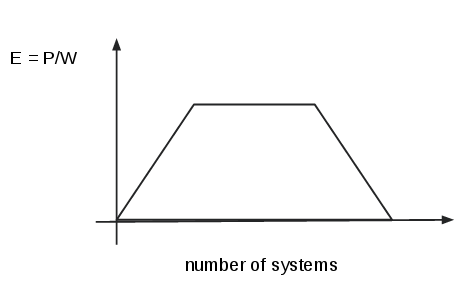
\includegraphics[width=0.75\textwidth]{images/graph_1.png}
\caption{Hypothesis of energy efficiency behaivor in embedded cluster}
\label{fig:4.1}
\end{figure}

\begin{figure}[H]
\centering
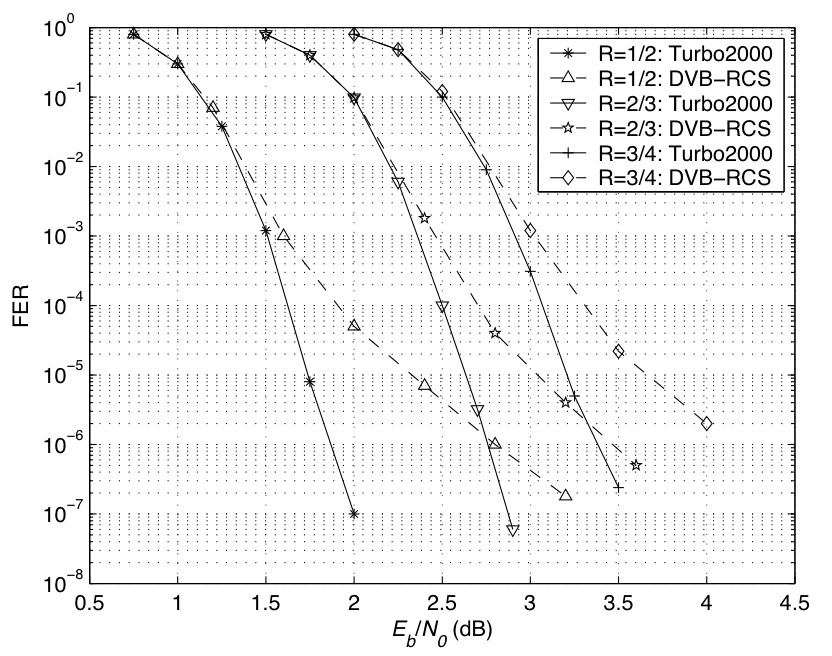
\includegraphics[width=0.7\textwidth]{images/figura4_2}
\caption{Comparaci'on del desempe'no de FER entre Turbo2000 y DVB-RCS. Par'ametros de la simulaci'on: Tama'no = 188 bytes, 8 iteraciones, q=4, QPSK y AWGN.}
\label{fig:4.2}
\end{figure}

\begin{figure}[H]
\centering
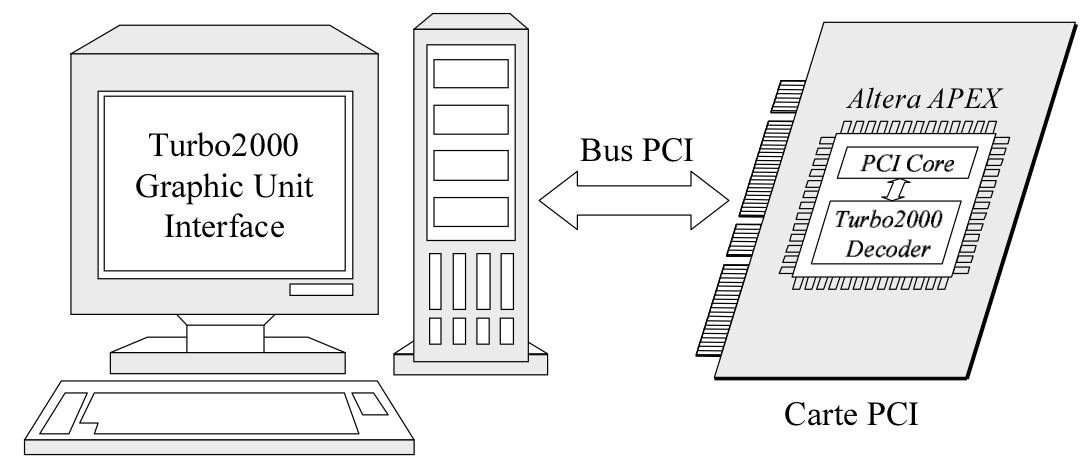
\includegraphics[width=0.9\textwidth]{images/figura4_3}
\caption{Plataforma Turbo2000.}
\label{fig:4.3}
\end{figure}

\section{Tablas}
\noindent
Esta secci'on presenta algunos ejemplos de formatos de tablas extra'idas de la referencia \cite{Demo:phdTesis} que se pueden usar en el documento de tesis.
\begin{table}[H]
	\begin{center}
		\begin{tabular}{ | c | c | c | }
			\hline
			& & \\[-18pt]
			\emph{q} bits	&	\emph{L}\subscript{max}	&	\begin{math}\Delta\end{math}\subscript{max} \\[3pt]
			\hline \hline
			& & \\[-18pt]
			2 & 11 & 8 \\[8pt]
			3 & 33 & 24 \\[8pt]
			4 & 77 & 82 \\[8pt]
			5 & 165 & 123 \\[8pt]
			6 & 341 & 395 \\[5pt]
			\hline
		\end{tabular}
	\end{center}
	\caption{Din'amica de m'etricas para diferentes valores de q con $R =1/2, E_b/N_0 = 2 dB$ y modulaci'on QPSK.}
\end{table}

\begin{table}[H]
	\begin{center}
	\begin{threeparttable}
	\begin{tabular}{ | c || c | c | }
		\hline
		& & \\[-8pt]
		Unit'e	&	\# Add./Soustr.	&	\# min(.)	\\[3pt]
		\hline \hline
		& & \\[-18pt]CMB			&	22					&	0					\\& & \\[-18pt]\hline
		& & \\[-18pt]Proc. ACS		&	$2^m \cdot N_a = 64$	&	$N_s \cdot (2^m-1)=48$	\\& & \\[-18pt]\hline
		& & \\[-18pt]CP			&	$2^m \cdot N_a = 64$	&	$2^m \cdot (N_s-1)=60$	\\& & \\[-18pt]\hline
		& & \\[-18pt]CIE\tnote{a}	&	$2^{m+1} = 8$		&	$2^m-1=3$			\\& & \\[-18pt]\hline
		& & \\[-18pt]CCD\tnote{b}	&	1					&	2					\\& & \\[-18pt]\hline
		& & \\[-18pt]CCA\tnote{b}	&	1					&	2					\\
		\hline
	\end{tabular}
	\setstretch{1.0}
	\begin{tablenotes}
		\item[\tiny a]{\tiny No se consideran los sub-bloques de actualizaci'on de los datos extr'insecos.}
		\item[\tiny b]{\tiny El comparador de salida es considerado como un sumador.}
	\end{tablenotes}
	\setstretch{1.5}
	\end{threeparttable}
	\end{center}
	\caption{Complejidad de c'alculo de las unidades del decodificador Turbo2000.}
\end{table}

\begin{table}[H]
	\begin{center}
	\begin{threeparttable}
	\begin{tabular}{ | l || l | l | l |}
		\hline
		& & & \\[-18pt]
		\textbf{Tratamiento}		&	\textbf{Unidades activas}		&	\textbf{\# Add./Soustr.}	&	\textbf{\# min(.)}	\\[3pt]
		\hline \hline
		& & &\\[-18pt]RETOUR 2	&	CMB, Proc. ACS \emph{Retour}&	$22+2^m \cdot N_s$			& $N_s \cdot (2^m-1)$\\& & &\\[-18pt]
		& & &\\[-18pt]			&						&	86						& 48\\& & &\\[-18pt]\hline
		& & &\\[-18pt]ALLER 2		&	CMB, Proc. ACS \emph{Aller},&	$22+2^{m+1} \cdot (N_s+1)$	& $N_s \cdot (2^m-1)-1$\\& & &\\[-18pt]
		& & &\\[-18pt]			&	CP, CIE				&	158						& 111\\& & &\\[-18pt]\hline
		& & &\\[-18pt]RETOUR 1	&	CMB, Proc. ACS \emph{Retour}&	$22+2^m \cdot N_s$			& $N_s \cdot (2^m-1)$\\& & &\\[-18pt]
		& & &\\[-18pt]			&						&	86						& 48\\& & &\\[-18pt]\hline
		& & &\\[-18pt]ALLER 1		&	CMB, Proc. ACS \emph{Aller},&	$24+2^{m+1} \cdot (N_s+1)$	& $N_s \cdot (2^m-1)+3$\\& & &\\[-18pt]
		& & &\\[-18pt]			&	CP, CIE, CDD, CCA			&	160						& 115\\[3pt]
		\hline
	\end{tabular}
	\end{threeparttable}
	\end{center}
	\caption{Complejidad de c'alculo seg'un el tratamiento del decodificador Turbo2000.}
\end{table}

\section{M'argenes}
\noindent
\begin{enumerate}
	\item El margen izquierdo (del lado del encuadernado) ser'a de tres cent'imetros, incluyendo tablas e ilustraciones. El margen derecho ser'a de dos cent'imetros.
	\item Los m'argenes superior e inferior ser'an de dos cent'imetros. Esto no incluye los encabezados o pies de p'agina.
	\item Las p'aginas horizontales deber'an tener en la parte superior de la hoja un margen de tres cent'imetros; para que, al ubicarlas de manera vertical en el manuscrito, este margen coincida con el requerido para el encuadernado.
\end{enumerate}

\section{Espacios}
\noindent
\begin{enumerate}
	\item El texto del trabajo se har'a a doble espacio como viene en este manual.
	\item Se permite usar espacio sencillo en el 'indice de contenido, de ilustraciones, de tablas y en los ap'endices.
	\item El espacio sencillo es obligatorio para citas textuales en p'arrafos de otros autores, pies de figura, pies de tabla y pies de p'agina. Ejemplo de una cita textual \cite{Demo:phdTesis}:\\
	
	\setstretch{1.0}
	\small
	``Un turbo-c'odigo m-binario est'a compuesto de dos c'odigos CRSC m-binarios id'enticos concatenados en paralelo a trav'es de un permutador. La t'ecnica de terminaci'on circular es utilizada en estos c'odigos bidimensionales para codificar bloques sin hacer uso de bits de terminaci'on. La tasa de codificaci'on global R para un turbo-c'odigo es igual a m/(m + 2).''
\end{enumerate}
\setstretch{1.5}

\section{P'aginas}
\noindent
\begin{enumerate}
	\item Se numeran todas las p'aginas a partir de las p'aginas de Dedicatoria, Agradecimientos, Resumen, Contenido, Lista de Tablas y Figuras, Bibliograf'ia, Ap'endices y Vitae.
	\item No se numeran las p'aginas de la Portada y de Firmas.
	\item Coloca los n'umeros de p'aginas en el centro del margen inferior al inicio de un cap'itulo, y en el margen superior derecho para las dem'as. Las p'aginas en las que aparecen cuadros y gr'aficas tambi'en deben numerarse y su disposici'on (vertical u horizontal) no debe alterar la posici'on del n'umero de p'agina.
	\item Las p'aginas que incluyen la Dedicatoria, Agradecimientos, Resumen, Contenido, Lista de Tablas y Figuras utilizan la numeraci'on romana, es decir, I, II, III, IV, etc.
	\item Las p'aginas a partir del cap'itulo 1 utilizan la numeraci'on ar'abiga, es decir, 1, 2, 3, etc. Esto considera tambi'en a la Bibliograf'ia, los Ap'endices y el Vitae.
	\item No uses la palabra ``p'agina'' antes de la numeraci'on de las p'aginas.
	\item Usa el mismo tipo de letra para todos los n'umeros de p'agina.
\end{enumerate}

\section{Manuscrito final del documento de tesis}
\noindent
El manuscrito final de tesis deber'a respetar el siguiente orden:
\begin{enumerate}
	\item Portada del empastado (obligatoria): No se coloca el n'umero de p'agina y no se cuenta. Ver primera p'agina del manual.
	\item P'agina de Firmas (obligatoria): No se coloca el n'umero de p'agina y no se cuenta. Ver segunda p'agina del manual.
	\item Dedicatoria (opcional): Se coloca p'agina con n'umero romano en min'uscula.
	\item Ep'igrafe (opcional): Se coloca p'agina con n'umero romano en min'uscula.
	\item P'agina de reconocimientos o agradecimientos (opcional): Se coloca p'agina con n'umero romano en min'uscula.
	\item Resumen (obligatorio): Se coloca p'agina con n'umero romano en min'uscula.
	\item 'Indice de contenido (obligatorio): Se coloca p'agina con n'umero romano en min'uscula.
	\item Lista de tablas (puede ser requerido): Se coloca p'agina con n'umero romano en min'uscula.
	\item Lista de ilustraciones o gr'aficas (puede ser requerido): Se coloca p'agina con n'umero romano en min'uscula.
	\item Lista de abreviaturas (opcional): Se coloca p'agina con n'umero romano en min'uscula.
	\item Glosario (opcional): Se coloca p'agina con n'umero romano en min'uscula.
	\item Introducci'on (obligatoria). La introducci'on ser'a considerada como el primer cap'itulo del cuerpo del manuscrito. A partir de aqu'i inicia la paginaci'on ar'abiga.
	\item Cuerpo del manuscrito (obligatorio): Continu'a la paginaci'on ar'abiga.
	\newpage
	\item Referencias bibliogr'aficas (obligatorio): Continu'a la paginaci'on ar'abiga. Utilizar el formato del IEEE como viene en la siguiente p'agina.
	\item Ap'endices (opcional): Continu'a la paginaci'on ar'abiga.
	\item Vitae (obligatorio): Continu'a la paginaci'on ar'abiga.
\end{enumerate}

\clearpage

	%Empieza configuracion de capitulo
\setstretch{1.0}
\titleformat{\chapter}[block]{\Large\bfseries}{CHAPTER \Huge\thechapter\vspace{25 pt}}{0 pt}{\\\fontsize{26}{36}\selectfont}
\titlespacing{\chapter}{0 pt}{30 pt}{50 pt}[0 pt]
\titleformat{\section}{\Large\bfseries}{\thesection}{0 pt}{\hspace{30 pt}}
\titleformat{\subsection}{\large\bfseries}{\thesubsection}{0 pt}{\hspace{30 pt}}
\pagestyle{fancy}
\fancyhead[LO,LE]{\footnotesize\emph{\leftmark}}
\fancyhead[RO,RE]{\thepage}
\fancyfoot[CO,CE]{}
%Termina configuracion de capitulo

\chapter{Experiments}
\setstretch{1.5} %Regresa el interlineado a 1.5

\normalsize
\noindent

\section{Find the correct OS}
\noindent

    The first approach was to find the correct Operating system for the test,
    however this wasn't easy in the beginning we started to create a few
    experiments. In the end we came up with a full support of MPi for embedded
    platforms support that the community thanks to us a lot.

    \subsection {Embedded Distributed Systems: A Case of Study with Clear Linux
    Project for Intel Architecture}
    \noindent



The main objective of this work will be to prove that a distributed embedded
system (Intel® Atom-TM Processor E3825) running real HPC workloads 
(MPI benchmarks) can be improved by the use of a customized operating system 



The need of more complex and smart applications (they must adapt their
performance as well as power) has risen the bar to create distributed systems
based on parallel embedded platforms. 

By definition: A distributed system consists of a collection of autonomous
computers, connected through a network and distribution middle-ware, which
enables computers to coordinate their activities and to share the resources of
the system, so that users perceive the system as a single, integrated computing
facility.

Advantages: 

\begin{enumerate} 
    
    \item \textbf{Partitioning Workload}: 
    By partitioning the workload onto multiple processors, 
    each processor is now responsible for only a fraction of the workload. 
    The processors can now afford to slow down by dynamic voltage scaling 
    (DVS) to run at more power-efficient states, and the degraded performance 
    on each processor can still contribute to an increased system-wide 
    performance by the increased parallelism.  

    \item \textbf{Heterogeneous HW}: 
    Another advantage with a distributed scheme is that heterogeneous hardware 
    such as DSP and other accelerators can further improve power efficiency 
    of various stages of the computation through specialization.

\end{enumerate}
 

Disadvantages: 

\begin{enumerate}
    \item \textbf{Network}: Despite the fact the distributed systems may have
    many attractive properties, they pay a higher price for message-passing 
    communications. Each node now must handle not only communication with 
    the external world, but also extra communication on the internal network. 
    As a result, even if the actual data payload is not large on an absolute 
    scale, the communication appears very expensive and does not scale to a few
    more nodes

    \item \textbf{Lack of optimized OS}: A typical embedded system often does
    not contain an operating system. Crafting distributed programs on such a
    bare-bone platform is extremely difficult and error-prone. Although many
    higher-level abstractions such as Message Passing Interfaces (MPI) have been
    proposed to facilitate distributed programming, these abstraction layers require
    extensive system resources with comprehensive operating systems support, which
    may not be available to an embedded platform 
    
\end{enumerate}
 
However in recent years we have seen an emergence of a new class of full-fledged
embedded systems (they are fully loaded with sufficient system resources as well
as networking and other peripheral devices, and a complete version of the
operating system with network support) In addition, they are typically designed
with power-management technology in order to extend the battery life

With these gaps closed there might be a chance to merge the parallel and
distributed paradigms on the embedded world.  A merging point of technologies
from different domains often inspires technology innovations in new domains.

\section{Development}

According to these in consideration there are multiple scenarios to test the
capability of an embedded distributed system: 


\begin{itemize} 
    
    \item Compare an Embedded system with generic SW (Linux base OS
    (Fedora/Ubuntu/Debian) and generic MPI protocol (MPICH)) against a
    regular development system (with the same OS and MPI tools)

    \item Compare an Embedded system with a distributed operating system
    against the same embedded system with custom SW (Linux from scratch system)


    \item Compare an Embedded system with a distributed operating system
    against the same embedded system with custom SW (Linux from scratch system and
    MPI for embedded (LMPI)) in order to check the gap in the multiple systems

\end{itemize}

For this report we will execute the experiment of the second scenario, due to the
fact that we have already done the study of the first scenario. In that case we
realize that despite the fact that the minnow Max ran 8 times slower than the
regular development system (NUC Haswell system) the Minnow Max was more stable
and with less drops in performance. 

The operating system we will use is the Fedora 19 system, the description of the
system is listed on the fedora project site home page (http://fedoraproject.org)

The benchmark we will use to measure the performance is MPIbench. This is a
program to measure the performance of some critical MPI functions. By critical
it means that the behavior of these functions can dominate the run time of a
distributed application. MP-Bench has now been integrated into LLCbench (Low
Level Characterization Benchmarks) 

The MPIfunctions that it stress are: 


\begin{itemize}

\item MPI\_Send/MPI\_Recv Bandwidth (Kb/second vs. bytes) 
\item MPI\_Send/MPI\_Recv Application latency or Gap time (us vs. bytes)
\item MPI\_Send/MPI\_Recv Roundtrip or 2 * Latency (trns/second vs. bytes) 
\item MPI\_Send/MPI\_Recv() BidirectionalBandwidth (Kb/second vs. bytes) 
\item MPI\_Bcast broadcast (Kb/second vs. bytes) 
\item MPI\_Reduce reduction (sum) (Kb/second vs. bytes) 
\item MPI\_AllReduce reduction (sum) (Kb/second vs. bytes) 
\item MPI\_Alltoall Each process sends to every other process (Kb/sec vs. bytes) 

\end{itemize}


    \subsection {Embedded Distributed Systems: A Case of Study with Yocto project}
    \noindent

\section{Find the correct MPI protocol configuration}
\noindent

\section{Embedded Distributed System: A case of study in smart greenhouses}
\noindent

\section{Embedded Distributed System: PnP measurement with comercial OS}
\noindent

\clearpage

	%Empieza configuracion de capitulo
\setstretch{1.0}
\titleformat{\chapter}[block]{\Large\bfseries}{CAP'ITULO \Huge\thechapter\vspace{25 pt}}{0 pt}{\\\fontsize{26}{36}\selectfont}
\titlespacing{\chapter}{0 pt}{30 pt}{50 pt}[0 pt]
\titleformat{\section}{\Large\bfseries}{\thesection}{0 pt}{\hspace{30 pt}}
\titleformat{\subsection}{\large\bfseries}{\thesubsection}{0 pt}{\hspace{30 pt}}
\pagestyle{fancy}
\fancyhead[LO,LE]{\footnotesize\emph{\leftmark}}
\fancyhead[RO,RE]{\thepage}
\fancyfoot[CO,CE]{}
%Termina configuracion de capitulo

\chapter{Conclusions}
\setstretch{1.5} %Regresa el interlineado a 1.5

\normalsize
\noindent

\section{Conclusions}
\noindent

In this thesis work it was proposed the hypothesis that a cluster of ultra-low
power IoT platforms can be as computing powerful and energy efficient as a
traditional computing system.

In chapter one we present a simulation to illustrate such hypothesis. It is described in
Figure~\ref{fig:1.2}.  At the beginning , the increment in the number of nodes
in the studied network produces an increment on performance; however, it is
expected to reach a maximum point at which power efficiency becomes stable and
it will remain in such state up to a certain point at which it will start to
decrease. 

As we can see in the previous graphs this behavior was achieved as expected. At
the number of platforms increases it is expected the performance benefit
increase, because the amount of work to be done is distributed among different
platforms, but as more are added due to the power they consume the performance
gain starts to minimize. When the ideal number of platforms is exceeded, the
power efficiency decrease rapidly.

In all the experiment we realize, the ideal number of platforms is always
between three and four. This gave us the confidence to say that as a conclusion
that the energy efficiency (using MPI Benchmarks as a reference workload) of an
IoT distributed system is similar to a traditional computing system \cite{NUC}
with three or four nodes.

\section{Future Work}
\noindent

\clearpage


	%Empieza configuracion
\setstretch{1.0}
\titleformat{\chapter}{\Huge\bfseries}{\thechapter}{0 pt}{\rule{340 pt}{3 pt}\\}
\titlespacing{\chapter}{100 pt}{-25 pt}{40 pt}[10 pt]	
\pagestyle{fancy}
\fancyhead[RO,RE]{\thepage}
\fancyfoot[CO,CE]{}
%Termina configuracion

\setstretch{1.5}
\nocite{Benkhelifa}

\nocite{Wun}

\bibliographystyle{includes/IEEEtranBST/IEEEtran}
\bibliography{includes/tesis}
\addcontentsline{toc}{chapter}{Bibliograf'ia}


	\appendix
	%Empieza configuracion de capitulo
\setstretch{1.0}
\titleformat{\chapter}[block]{\Large\bfseries}{AP'ENDICE \Huge\thechapter\vspace{25 pt}}{0 pt}{\\\fontsize{26}{36}\selectfont}
\titlespacing{\chapter}{0 pt}{30 pt}{50 pt}[0 pt]
\titleformat{\section}{\Large\bfseries}{\thesection}{0 pt}{\hspace{30 pt}}
\titleformat{\subsection}{\large\bfseries}{\thesubsection}{0 pt}{\hspace{30 pt}}
\pagestyle{fancy}
\fancyhead[LO,LE]{\footnotesize\emph{\leftmark}}
\fancyhead[RO,RE]{\thepage}
\fancyfoot[CO,CE]{}
%Termina configuracion de capitulo

\chapter{Procedimientos de Defensa de la Propuesta} %Cambia al nombre de tu capitulo
\setstretch{1.5} %Regresa el interlineado a 1.5

\normalsize
Una vez que se ha redactado la propuesta, debe entregarla al director para que la firme. Se recomienda hacer dos copias del documento, una para usted y otra para la direcci'on de maestr'ia.

	%Empieza configuracion de capitulo
\setstretch{1.0}
\titleformat{\chapter}[block]{\Large\bfseries}{AP'ENDICE \Huge\thechapter\vspace{25 pt}}{0 pt}{\\\fontsize{26}{36}\selectfont}
\titlespacing{\chapter}{0 pt}{30 pt}{50 pt}[0 pt]
\titleformat{\section}{\Large\bfseries}{\thesection}{0 pt}{\hspace{30 pt}}
\titleformat{\subsection}{\large\bfseries}{\thesubsection}{0 pt}{\hspace{30 pt}}
\pagestyle{fancy}
\fancyhead[LO,LE]{\footnotesize\emph{\leftmark}}
\fancyhead[RO,RE]{\thepage}
\fancyfoot[CO,CE]{}
%Termina configuracion de capitulo

\chapter{'Ultimos Detalles} %Cambia al nombre de tu capitulo
\setstretch{1.5} %Regresa el interlineado a 1.5

\normalsize
Aqu'i vienen los detalles que no se mencionaron en el cuerpo del contenido para alg'un tema espec'ifico.

	%Empieza configuracion
\setstretch{1.0}
\titleformat{\chapter}{\Huge\bfseries}{\thechapter}{0 pt}{\rule{340 pt}{3 pt}\\}
\titlespacing{\chapter}{100 pt}{-25 pt}{40 pt}[10 pt]	
\pagestyle{fancy}
\fancyhead[RO,RE]{\thepage}
\fancyfoot[CO,CE]{}
%Termina configuracion

\chapter*{Vitae}
\addcontentsline{toc}{chapter}{Vitae}
\setstretch{1.5} %Regresa el interlineado a 1.5

\normalsize
\noindent

\end{document}
